\documentclass[12pt, a4paper, oneside]{ctexart}
\usepackage{amsmath, amsthm, amssymb, appendix, bm, graphicx, hyperref, mathrsfs, graphicx}
\usepackage{authblk}
% \usepackage[perpage]{footmisc}
\usepackage{multirow}
\usepackage{hyperref}
\hypersetup{hidelinks,
	colorlinks=true,
	allcolors=black,
	pdfstartview=Fit,
	breaklinks=true}
\usepackage{float}
\usepackage{enumerate}

\linespread{1.5}

\renewcommand{\abstractname}{\Large\textbf{绪言}}
\newcounter{parnum}[section]
\newcommand{\N}{%
   \noindent\refstepcounter{parnum}%
    \makebox[\parindent][l]{\textbf{\arabic{parnum}.}}}
% Use a generous paragraph indent so numbers can be fit inside the
% indentation space.
\setlength{\parindent}{2em}

\begin{document}

\setcounter{page}{0}
\begin{center}
	\Large{\textbf{圣.奥古斯丁忏悔录}} \\ \vspace{1em}
	\small{\href{https://faculty.georgetown.edu/jod/augustine/conf.pdf}{The Confessions of Saint Augustine}} \\ \vspace{2em}
	\small{原著:Saint Augustine} \\ \vspace{1em}
	\small{译者:Job Zhao} \\ \vspace{1em}
	\small{编译日期: \today} \\ \vspace{1em}
	\small{Version 1.00} \\ \vspace{1em}
\end{center}
\vfill
\vspace{20em}
\begin{tabular*}{\textwidth}{cc}
	\includegraphics{figure/by-nc.eps}
	& \begin{minipage}[b]{0.6\textwidth}
		\footnotesize
		本作品采用知识共享署名-非商业性使用4.0国际许可协议进行许可。访问\url{http://creativecommons.org/licenses/by-nc/4.0/ }查看该许可协议。
	\end{minipage}
\end{tabular*}
\vspace{2mm}
\thispagestyle{empty}

\newpage

\begin{abstract}
	感谢主!让我与圣.奥古斯丁相遇。

	他是领我进入信仰的第一也是唯一一人。正是三年前我在读他的《自由意志》时被感召,立志离弃罪恶,跟随基督。如今我已受洗而与这位圣徒之间有了团契。而现有圣.奥古斯丁作品的译本已无法满足我与他交契的需要,我渴望能更进一步,通过自己翻译他的文字与他交通,由这位圣徒受上帝灵感而发的话语引领我,到离祂更近的地方。

	% 想到这里,突然觉得自己缺了什么。我本打算以Albert C. Outler的英译本为底本,参考其他英译本来完成翻译。因为在开始这项工作时,我对拉丁语一窍不通。但翻译英译本,怎么叫与他更进一步的交通呢?这不也是自欺吗?于是,我修改了我的计划---我将边学习拉丁语,边进行翻译。初稿的翻译依旧以英译本为基础。而等到初稿完成,希望我能在第二遍校对时,尝试阅读拉丁原文进行修正,而更接近圣.奥古斯丁。
	
	这是这位圣徒的忏悔,也是我的忏悔。
	
	\hfill Job Zhao

	\hfill 2024年10月11日
    
\end{abstract}

\newpage
\pagenumbering{Roman}
\setcounter{page}{1}
\tableofcontents
\newpage
\setcounter{page}{1}
\pagenumbering{arabic}

\section*{介绍}


\newpage

% BOOK ONE
\section{卷一}

% In God’s searching presence, Augustine undertakes to plumb the depths of his memory to trace the mysterious pilgrimage of grace which his life has been--and to praise God for his constant and omnipotent grace. In a mood of sustained prayer, he recalls what he can of his infancy, his learning to speak, and his childhood experiences in school. He concludes with a paean of grateful praise to God.
在上帝搜索的现状中,奥古斯丁着手探寻他的记忆深处,追溯他生命已走过的神秘的恩典朝圣之旅---并为祂恒常而万能的恩典赞美上帝。在一种经久祷告的情绪中,他回忆他所能回忆的幼年、他学习说话以及他在学校的童年经历。他以一首对上帝感激的赞美颂歌来结尾。

%  CHAPTER I
\subsection{第一章}

% magnus es, domine, et laudabilis valde. magna virtus tua et sapientiae tuae non est numerus. 
\N “主啊,祢是伟大的,而要被极大地赞美;祢的权柄巨大,而祢的智慧无限。”
	\footnote {
		\href{https://biblehub.com/psalms/96-4.htm}{诗96:4} 因为耶和华是伟大的,而最值得赞美;祂要在所有诸神之上被敬畏。
		\href{https://biblehub.com/psalms/48-1.htm}{诗48:1} 一首歌。可拉之子的诗篇。耶和华是伟大的而最值得赞美,在我们的上帝之城,祂的圣山中。
		\href{https://biblehub.com/psalms/145-3.htm}{诗145:3} 耶和华是伟大的,而最值得赞美;祂的伟大无人能洞悉。
		\href{https://biblehub.com/psalms/147-5.htm}{诗147:5} 我们的主是伟大的且权柄强大;祂的理解力没有极限。
        \href{https://biblehub.com/1_corinthians/1-24.htm}{林前1:24} 但对那些上帝已召唤的人,犹太人和希腊人兼有,基督都是上帝的大能和上帝的智慧。
	}
	% et laudare te vult homo, aliqua portio creaturae tuae, et homo circumferens mortalitatem suam, circumferens testimonium peccati sui et testimonium quia superbis resistis; et tamen laudare te vult homo, aliqua portio creaturae tuae.
	而人---祢创世的一小部分---渴望赞美祢;他周身承受他的必朽伴着他,并携带他罪恶的证据和祢抗拒骄傲的证明。
	\footnote {
		\href{https://biblehub.com/proverbs/3-34.htm}{箴3:34} 祂嘲笑骄傲的嘲笑者,但向谦卑和受压迫者展示恩惠。
		\href{https://biblehub.com/1_peter/5-5.htm}{彼前5:5} 以相同的方法,你们这些更年轻的,使你们自己服从于你们的长者。你们所有人,都用互相间的谦卑穿戴你们自己,因为 “上帝反对骄傲的人,却向谦卑的人展示恩惠。”
	}
	他仍然渴望赞美祢,尽管这人仅仅是祢创世的一小部分。
	% tu excitas ut laudare te delectet, quia fecisti nos ad te et inquietum est cor nostrum donec requiescat in te.
	祢已唤起他,以致他应乐于赞美祢,因为祢已为祢自己造了我们,而我们的心不安歇直到它达到而安息在祢里面。
	% da mihi, domine, scire et intellegere utrum sit prius invocare te an laudare te, et scire te prius sit an invocare te.
	主啊,请赐予我认识并理解是首先祈求祢还是首先赞美祢;是先认识祢还是先求靠祢。
    \footnote {
		\href{https://biblehub.com/psalms/119-34.htm}{诗119:34} 请赐予我理解,以致我能保持祢的律法并以我所有的心遵守它。
        \href{https://biblehub.com/psalms/105-1.htm}{105:1} 将赞美献给耶和华,求靠祂的名;在列邦中间揭晓祂已完成的。
	}
	% sed quis te invocat nesciens te? aliud enim pro alio potest invocare nesciens.
	但谁能祈求祢,却不认识祢呢?因为他不认识祢,就可能将祢作为不是祢的另一个来祈求。
	% an potius invocaris ut sciaris?quomodo autem invocabunt, in quem non crediderunt?aut quomodo credent sine praedicante?
	或许我们应该祈求祢以使我们能到达认识祢?但“他们尚不信祂,怎么会求靠祂呢?或者没有传道人,他们怎么会信呢?”
	\footnote {
		\href{https://biblehub.com/romans/10-14.htm}{罗10:14} 那么,他们怎么能求靠他们未相信的那一位呢?而他们怎么能相信他们未听过的人呢?而没有人向他们传讲,他们怎么能听见呢?
	}
	% et laudabunt dominum qui requirunt eum: quaerentes enim inveniunt eum et invenientes laudabunt eum.
	现在,“他们寻求祂,就会赞美主,”
	\footnote {
		\href{https://biblehub.com/psalms/22-26.htm}{诗22:26} 穷人会吃并被满足;那些寻求耶和华的人会赞美他---愿你们的心永远活着!
	}
	因为 “那些寻求的人就会找到祂,”
	\footnote {
		\href{https://biblehub.com/matthew/7-7.htm}{太7:7} “问求,它就会被赐给你;寻求,你就会找到;敲门,门就会向你被敞开。
	}
	而,找到祂,就会赞美祂。
    % quaeram te, domine, invocans te et invocem te credens in te: praedicatus enim es nobis.
    主啊,我将通过求靠祢来探求祢,而我会通过信仰祢来求靠祢:因为祢已真确地被传讲给我们。
    \footnote {
		\href{https://biblehub.com/jeremiah/29-11.htm}{耶29:11} 因为我知道我对你们有的计划,”耶和华宣告,“是使你们兴旺的计划,而不是伤害你们的,是赐给你们希望和一个未来的计划。
        \href{https://biblehub.com/jeremiah/29-12.htm}{12} 于是你们会求靠我,而来向我祷告,而我会听你们。”
        \href{https://biblehub.com/romans/10-15.htm}{罗10:15} 而除非他们被差派,任何人怎么能传讲呢?如经上所记:“那些带来佳音的人的脚是多么美丽!”
        \href{https://biblehub.com/philippians/1-18.htm}{腓1:18} 但这有什么关系呢?重要的是,以每种方法,无论出自虚假的动机或真正的,基督都被传讲。而因如此,我欣喜。是的,并且我会持续欣喜,
	}
	% invocat te, domine, fides mea, quam dedisti mihi, quam inspirasti mihi per humanitatem filii tui, per ministerium praedicatoris tui.
	主啊,我的信心应求靠祢,它是祢已赐予的,并且祢用它已启发我,藉着祢圣子的人性,
    \footnote {
		言成肉身是启示的根本原理。
	}
    并藉着祢的传道人的事工。
	\footnote {
		这里可能指米兰的安布罗斯主教;见第五卷:第十三章;第八卷:第十一章-第3节。但也有研究认为可能指使徒保罗,或者是基督本身。
	}

%  CHAPTER II
\subsection{第二章}

% et quomodo invocabo deum meum, deum et dominum meum, quoniam utique in me ipsum eum vocabo, cum invocabo eum?
\N 而我要如何求靠我的上帝---我的上帝和我的主呢?因为当我求靠祂时,我肯定呼唤祂进入我里面。
	% et quis locus est in me quo veniat in me deus meus, quo deus veniat in me, deus qui fecit caelum et terram?
	而在我里面有什么地方我的上帝能进来呢?上帝,那创造了天与地的上帝,
    \footnote {
		\href{https://biblehub.com/genesis/1-1.htm}{创1:1} 起初,上帝创造诸天与地。
	}
    能进入到我里面何处呢?
    % itane, domine deus meus? est quicquam in me quod capiat te? an vero caelum et terra, quae fecisti et in quibus me fecisti, capiunt te?
    是吗?主我的上帝啊,在我里面是否有任何东西容纳祢?或者祢已创造的那天与那地---在其中祢也创造了我---是否确实容纳祢?
	% an quia sine te non esset quidquid est, fit ut quidquid est capiat te?
	是否可能,既然没有祢,无物会是其存在,那么祢使它如此而无论任何存在都有某种容量来接收祢?
	% quoniam itaque et ego sum, quid peto ut venias in me, qui non essem nisi esses in me?
	既然因此我也存在,而且除非祢在我里面,我就不能存在,那么,为什么我企求祢进到我里面来?
	% non enim ego iam inferi, et tamen etiam ibi es, nam etsi descendero in infernum, ades.
	因为毕竟,我现在不属于地狱---而就算如此祢也在那里,因为“如果我下到地狱中,祢在那里。”
	\footnote {
		\href{https://biblehub.com/psalms/139-8.htm}{诗139:8} 如果我升上到诸天,祢在那里;如果我在诸渊铺我的床,祢在那里。
	}
	% non ergo essem, deus meus, non omnino essem, nisi esses in me. an potius non essem nisi essem in te, ex quo omnia, per quem omnia, in quo omnia? etiam sic, domine, etiam sic.
	因此,我的上帝,我不会存在---我会根本没有任何存在---除非祢在我里面。
    或者相反,除非我在祢里面否则我不会存在?而万物都源自祢,藉着祢且在祢里面。
    \footnote {
		\href{https://biblehub.com/romans/11-36.htm}{罗11:36} 因为万物都源自祂,而藉着祂,并为了祂。荣耀永远归于祂!阿门。
        \href{https://biblehub.com/1_corinthians/8-6.htm}{林前8:6} 但对我们,有且惟有一位上帝,圣父,万物都从祂而来,而我们为祂而活;并且有且仅有一位主,耶稣基督,万物都藉着祂而来,而我们藉着祂而活。
	}
    正是如此,主啊,正是如此。
	% quo te invoco, cum in te sim? aut unde venias in me? quo enim recedam extra caelum et terram, ut inde in me veniat deus meus, qui dixit, `caelum et terram ego impleo'?
	当我早已在祢里面,我呼唤祢到哪里呢?或者祢会从哪里进到我里面来?超越天与地之外,我能去哪里,以致在那我的上帝能临到我---祂曾说,“我充满天与地”?
	\footnote {
        \href{https://biblehub.com/jeremiah/23-23.htm}{耶23:23} “难道我仅是一个附近的上帝,”耶和华宣告:“而不是一个遥远的上帝吗?
		\href{https://biblehub.com/jeremiah/23-24.htm}{24} 谁能躲藏在隐秘的地方,以致我不能看见他们呢?”耶和华宣告。“我难道不是充满天地吗?”耶和华宣告。
	}

% CHAPTER III
\subsection{第三章}

% capiunt ergone te caelum et terra, quoniam tu imples ea? an imples et restat, quoniam non te capiunt?
\N 那么,既然祢充满这天与地,它们是否容纳祢?或者,祢是否充满并从它们溢出,因为它们不能容纳祢?
	\footnote {
		\href{https://biblehub.com/1_kings/8-27.htm}{王上8:27} “但上帝真正会栖居在地上吗?诸天,即使是至高的天国,也无法容纳你。我建成的这神殿,是多么渺小!
	}
    % et quo refundis quidquid impleto caelo et terra restat ex te?
	而天与地满了后,祢在哪里倾倒出那些祢余下的呢?
    % an non opus habes ut quoquam continearis, qui contines omnia, quoniam quae imples continendo imples?
	或者,祢包含万物,是否就没有需要应被任何包含,因为那些祢充满的,祢由包含它们来充满?
	% non enim vasa quae te plena sunt stabilem te faciunt, quia etsi frangantur non effunderis.
	不要以为是充满祢的器皿使祢稳固,因为即使它们破碎了,祢也不会被倾倒出来。
	% et cum effunderis super nos, non tu iaces sed erigis nos, nec tu dissiparis sed conligis nos.
	而,当祢被倾倒在我们之上,祢没有由此被放倒;反而我们被抬升。
    \footnote {
		\href{https://biblehub.com/acts/2-17.htm}{徒2:17} “‘在这末后的日子,上帝说,我会将我的灵倾倒在所有子民上。你们的儿子们和女儿们会说神启,你们的年轻人会看见异象,你们的老人会梦见梦境。
		\href{https://biblehub.com/acts/2-18.htm}{18} 甚至在那些日子,我会将我的灵倾倒在我的仆人上,男人和女人兼有,而他们会说神启。
        \href{https://biblehub.com/isaiah/44-3.htm}{赛44:3} 因为我会将水倒在干渴的土地上,并将溪流倒在干旱的地面上;我会将我的灵倾倒在你的孩子上,并将我的祝福倾倒在你的后代上。
        \href{https://biblehub.com/psalms/146-8.htm}{诗146:8} 耶和华将视力赐给盲目的人,耶和华将那些俯伏的人抬起,耶和华爱义人。
	}
	祢也没有被分散;相反,祢将我们聚集在一起。
    \footnote {
        \href{https://biblehub.com/isaiah/11-12.htm}{赛11:12} 祂会为列邦拉起一块横幅,并聚集以色列的流亡者;祂会从大地的四方聚集被分散的犹大子民。
        \href{https://biblehub.com/psalms/147-2.htm}{诗147:2} 耶和华造就耶路撒冷;祂聚集以色列的流亡者。
	}
    % sed quae imples omnia, te toto imples omnia.
	但当祢充满万物,祢用祢整个存有充满它们所有。
	% an quia non possunt te totum capere omnia, partem tui capiunt et eandem partem simul omnia capiunt?
	或者,既然甚至万物都不能够完全容纳祢,是否它们只容纳祢的一部分而万物在同时都容纳祢那相同的部分?
	% an singulas singula et maiores maiora, minores minora capiunt?
	或者,是否单个体单独地容纳祢?而较大的事物容纳祢较多,而较小的事物则较少?
	% ergo est aliqua pars tua maior, aliqua minor? an ubique totus es et res nulla te totum capit?
	% 或者,是否不是如此,而是祢在每个地方都是全然呈现,而以这样一种方法就没有东西全然容纳祢?
	而如此,是否祢某些部分较大,某些部分较小?或者,祢在任何地方都是全然呈现,以致无物全然容纳祢?

% CHAPTER IV
\subsection{第四章}

% quid es ergo, deus meus? quid, rogo, nisi dominus deus? quis enim dominus praeter dominum? aut quis deus praeter deum nostrum? 
\N 因此,我的上帝是什么?如果不是主上帝,我问求什么呢?“因为除了主祂自己,谁是主?或者除了我们的上帝,谁是上帝呢?”
	\footnote {
        \href{https://biblehub.com/psalms/18-31.htm}{诗18:31} 因为除耶和华之外,谁是上帝?而除了我们的上帝,谁是那磐石呢?
	}
	% summe, optime, potentissime, omnipotentissime, misericordissime et iustissime, secretissime et praesentissime, pulcherrime et fortissime, stabilis et incomprehensibilis, immutabilis mutans omnia, numquam novus numquam vetus, innovans omnia et in vetustatem perducens superbos et nesciunt.
	至高,
    \footnote {
        \href{https://biblehub.com/psalms/83-18.htm}{诗83:18} 让他们知道祢,祢的名是耶和华---惟独祢是全地之上的至高者。
	}
    至善,
    \footnote {
		\href{https://biblehub.com/psalms/119-68.htm}{诗119:68} 祢是善良的,而祢所做的是善的;请教导我祢的预旨。
	}
    至能,
    \footnote {
		\href{https://biblehub.com/psalms/45-3.htm}{诗45:3} 大能者啊,束紧祢的剑;用光辉和威严穿戴祢自己。
	}
    至全能;
    \footnote {
		\href{https://biblehub.com/genesis/17-1.htm}{创17:1} 亚伯兰九十九岁时,耶和华向他显现并说:“我是全能的上帝;要信实地走在我面前,并无可指摘。
		\href{https://biblehub.com/revelation/4-8.htm}{启4:8} 这四个活物每个都有六个翅膀,遍体甚至在它的翅膀下都被眼睛覆盖。它们昼夜永不停止说:“‘圣哉,圣哉,圣哉是主--全能的上帝’,祂昔在、而今在、并且将在要来。”
	}
    至仁而至公;
    \footnote {
        \href{https://biblehub.com/exodus/34-6.htm}{出34:6} 而祂从摩西前面经过,宣布着:“耶和华,耶和华,怜悯而仁慈的上帝,不轻易发怒,满溢着爱和信实,
		\href{https://biblehub.com/nehemiah/9-33.htm}{尼9:33} 在对我们已发生的所有上,祢已留存正义;祢已信实行事,而我们却行事邪恶。
        \href{https://biblehub.com/psalms/116-5.htm}{诗116:5} 耶和华仁慈而正义;我们的上帝满有怜悯。
	}
    至隐秘而至同现;
    \footnote {
        \href{https://biblehub.com/deuteronomy/29-29.htm}{申29:29} 隐秘的事情属于耶和华我们的上帝,但被启示的事情永远属于我们和我们的子女,使我们能遵循这律法所有的言词。
        \href{https://biblehub.com/matthew/28-20.htm}{太28:20} 并教导他们遵守我已命令你们的一切。而无疑我总是与你们同在,到这时代的最末了。
	}
    至美而至强;
    \footnote {
        \href{https://biblehub.com/psalms/96-6.htm}{诗96:6} 光辉和威严在祂面前;力量和美丽充满祂的圣殿。
        \href{https://biblehub.com/jeremiah/32-18.htm}{耶13:18} 祢向千万的人展示爱,而为那父母的罪恶将惩罚带到他们之后他们的儿女的膝中。伟大而强力的上帝,祢的名是万军之耶和华,
	}
    稳定,却无法掌握;
    \footnote {
        \href{https://biblehub.com/psalms/90-2.htm}{诗90:2} 在山脉出生或在你生出整个世界之前,你是上帝,从永久到永久。
		\href{https://biblehub.com/1_timothy/1-17.htm}{提前1:17} 现在将尊贵与荣耀归给永恒、不朽、不可见的国王、惟一的上帝,直到永永远远。阿门。
        \href{https://biblehub.com/john/1-5.htm}{约1:5} 那光在黑暗中照耀,而黑暗未曾胜过祂。
		\href{https://biblehub.com/romans/11-33.htm}{罗11:33} 深哉,上帝智慧和知识的丰富!祂的判断何其难测,而祂的路径超出追踪!
        \href{https://biblehub.com/job/9-10.htm}{伯9:10} 祂实行无法洞悉的奇事、无法数算的奇迹。
	}
    不可改变,却改变万物;
    \footnote {
        \href{https://biblehub.com/james/1-17.htm}{雅1:17} 每一份善而完美的恩赐都源自上天,从天国众光之父降临,而祂不会像飘移的阴影一样改变。
		\href{https://biblehub.com/malachi/3-6.htm}{玛3:6} “我耶和华不改变。所以你们,雅各的后代,不被摧毁。
        \href{https://biblehub.com/revelation/21-5.htm}{启21:5} 祂落座在宝座上说:“我正在使一切变新!”然后祂说:“将此记下,因为这些言词是可信且永真的。”
	}
    从未新,从未老;
    \footnote {
        \href{https://biblehub.com/hebrews/13-8.htm}{来13:8} 耶稣基督昨天和今天且永远是一样的。
	}
    使万物变新,却带给骄傲者暮年,他们却不知道;
    \footnote {
        \href{https://biblehub.com/jobs/9-5.htm}{伯9:5} 祂移动山脉,而它们不知道;并在愤怒中颠覆它们。
	}
    % semper agens semper quietus, conligens et non egens, portans et implens et protegens, creans et nutriens et perficiens, quaerens cum nihil desit tibi.
    总是工作,却不断安歇;
    \footnote {
        \href{https://biblehub.com/john/5-17.htm}{约5:17} 耶稣回答他们说:“我父总是在做祂的工作到即日,而我也在工作。”
        \href{https://biblehub.com/1_chronicles/23-25.htm}{代上23:25} 因为大卫已说过:“因为耶和华,以色列的上帝,已准予祂的子民安息并已来到在耶路撒冷永远栖居,
	}
    聚集,却什么都不需要;
	\footnote {
        \href{https://biblehub.com/acts/17-25.htm}{徒17:25} 而且祂不被人手侍奉,仿佛祂需要任何东西。相反,祂本身赐给每个人生命与呼吸以及其他一切。
	}
	维持,充盈,并保护;
    \footnote {
        \href{https://biblehub.com/hebrews/1-3.htm}{来1:3} 圣子是上帝荣耀的光辉,是祂存有的精确表征,由祂大能的言维持万物。在祂已为罪恶提供净化之后,祂定坐在了天国中至威者的右手边。
        \href{https://biblehub.com/2_thessalonians/3-3.htm}{帖后3:3} 但主是信实的,而且祂会坚固你们,并保护你们避开恶魔。
	}
    创造,滋养,并臻备;
    \footnote {
        \href{https://biblehub.com/1_peter/5-7.htm}{彼前5:7} 将你们所有的焦虑都抛给祂,因为祂护理你们。
        \href{https://biblehub.com/proverbs/16-4.htm}{箴16:4} 耶和华使一切都运行出它恰当的目的---甚至有恶人为灾难的一天。
	}
    搜寻,而却什么都不缺乏。
	\footnote {
        \href{https://biblehub.com/ezekiel/34-16.htm}{结34:16} 我会寻找丢失的人并将迷失的人带回。我会包扎伤者并使弱者坚固,但圆滑而要强者我会毁灭。我会以公正牧养羊群。
	}
	% amas nec aestuas, zelas et securus es, paenitet te et non doles, irasceris et tranquillus es, opera mutas nec mutas consilium, recipis quod invenis et numquam amisisti.
	祢爱,但没有情感;
    \footnote {
        \href{https://biblehub.com/1_john/4-8.htm}{约壹4:8} 任何不去爱的人就不认识上帝,因为上帝是爱。
		\href{https://biblehub.com/1_john/4-16.htm}{16} 而所以我们知道并依靠上帝对我们有的爱。上帝是爱。无论谁活在爱里都活在上帝里面,而且上帝就在他们里面。
		\href{https://biblehub.com/acts/14-11.htm}{徒14:11} 当人群看见保罗已做的,他们就用吕高尼亚语大喊:“诸神已以人形降临到我们!”
		\href{https://biblehub.com/acts/14-15.htm}{15} “朋友们,你们为什么在做这?我们也只是(有情感的)人类,像你们一样。我们正将福音带给你们,告诉你们要转离这些毫无价值的东西,而归向创造天与地与海及在其中一切的永活的上帝。
	}
    忌邪,却无所牵挂;
    \footnote {
        \href{https://biblehub.com/joel/2-18.htm}{珥2:18} 于是耶和华对祂的土地忌邪,而怜惜祂的子民。
        \href{https://biblehub.com/exodus/34-14.htm}{出34:14} 不要敬拜别的神,因为耶和华,祂的名叫忌邪,是一位忌邪的上帝。
        \href{https://biblehub.com/psalms/88-5.htm}{诗88:5} 我与死人一同被置留,像那些躺在坟墓里的被残杀者,祢不再记念他们,他们被切断祢的关心。
	}
    悔改而没有懊悔;
    \footnote {
        \href{https://biblehub.com/genesis/6-6.htm}{创6:6} 耶和华后悔祂在地上已制造的人类物种,而祂的心被深深地烦恼。
        \href{https://biblehub.com/genesis/6-7.htm}{7} 所以耶和华说:“我会从地表擦除我已创造的人类种族---和与他们一同的动物、鸟类和在地面活动的受造物,因为我后悔我已制造他们。”
	}
    愤怒,却依旧宁静。
    \footnote {
        \href{https://biblehub.com/exodus/4-14.htm}{出4:14} 于是耶和华的愤怒向摩西燃烧,而祂说:“你的兄弟利未人亚伦如何呢?我知道他能讲得很好。他已经在会见你的路上,而他会很高兴见到你。
	}
	祢改变祢的运作,而不改变祢的旨意;
    \footnote {
        \href{https://biblehub.com/1_corinthians/12-6.htm}{林前12:6} 有不同种类的运作,但在它们所有中及在每个人中,都是同一个上帝在做工。
        \href{https://biblehub.com/hebrews/6-17.htm}{来6:17} 因为上帝想使祂旨意的不变性对被应许了的继承人非常清晰,祂就以一个誓言确认了它。
	}
    祢恢复祢找到的,而永未丢失。
    \footnote {
        \href{https://biblehub.com/isaiah/58-12.htm}{赛58:12} 祢的子民将重建古老的废墟,并兴起悠久的根基;祢会被称为断壁的修复者,栖居街道的恢复者。
        \href{https://biblehub.com/luke/15-4.htm}{路15:4} “假设你们其中一个有一百只羊而丢失其中一只。难道他不把这九十九只留在旷野上而去追寻那丢失的羊,直到他找到它吗?
	}
	% numquam inops et gaudes lucris, numquam avarus et usuras exigis, supererogatur tibi ut debeas: et quis habet quicquam non tuum?
	祢从未贫乏但祢仍为收益欣喜;
    \footnote {
		\href{https://biblehub.com/luke/15-7.htm}{路15:7} 我告诉你们,以相同的方法,比起九十九个不需要悔改的义人,在天国中为一个悔改的罪人会有更多的欢喜。
        \href{https://biblehub.com/matthew/25-21.htm}{太25:21} “他的主人回复:‘干得好,善良而信实的仆人!你已在少许事上信实;我会让你负责许多事情。过来并分享你主人的幸福!’
	}
    从未贪心,却索求利息。
	\footnote {
		\href{https://biblehub.com/matthew/25-27.htm}{太25:27} 那好,你们本应将我的钱与银行家储蓄,以致当我返回时,我就会将它与利息一同收回。
        参见\href{https://biblehub.com/niv/matthew/25.htm}{太25:14-30金袋的比喻。}
	}
	人们付酬过度以致祢成为欠债人;
    \footnote {
		\href{https://biblehub.com/luke/10-35.htm}{路10:35} 第二天,他拿出两个银币并将它们交给旅店老板。‘请照看他,’他说,“而我回来时,我会为你可能有的额外开销补偿你。’
	}
    但究竟谁拥有不属于祢的任何东西呢?
    \footnote {
		\href{https://biblehub.com/1_corinthians/4-7.htm}{林前4:7} 因为谁使你们与任何其他人不同呢?你们有什么是未领受了的呢?而如果你们确实领受了它,为什么你们夸耀如同你们没有呢?
	}
	% reddis debita nulli debens, donas debita nihil perdens. et quid diximus, deus meus, vita mea, dulcedo mea sancta, aut quid dicit aliquis cum de te dicit?
	祢什么都不欠人的,却向他们偿清债务,而当祢取消债务时,祢并未因此失去任何东西。
    \footnote {
		\href{https://biblehub.com/matthew/6-12.htm}{太6:12} 并对我们饶恕我们的债,如同我们也已饶恕我们的欠债人。
	}
	但,我的上帝,我的生命,
    \footnote {
		\href{https://biblehub.com/john/11-25.htm}{约11:15} 耶稣告诉她:“我是复活和生命。任何信仰我的人会存活,甚至在死之后。
        \href{https://biblehub.com/john/14-6.htm}{14:6} 耶稣回答:“我是道路、真理和生命。除非藉着我,就无人到圣父这里来。
	}
    我神圣的甘饴啊,
    \footnote {
		\href{https://biblehub.com/psalms/68-10.htm}{诗68:10} 祢的子民定居在它里面,而上帝啊,源自祢的丰惠,祢供养穷人。
	}
    我已所说的这是什么呢?
    % et vae tacentibus de te, quoniam loquaces muti sunt.
    当任何人谈论祢时,他能说什么呢?但对祢静默的人有祸了
    \footnote {
		\href{https://biblehub.com/psalms/32-3.htm}{诗32:3} 当我保持静默时,我的骨头因着我终日叹息而消磨。
	}
    ---因为那些最健谈的人却无话可说。
    \footnote {
		\href{https://biblehub.com/proverbs/10-19.htm}{箴10:19} 罪恶不被言词倍增终结,而审慎的人守住他们的舌头。
	}

% CHAPTER V
\subsection{第五章}

% quis mihi dabit adquiescere in te? 
\N 谁会准予我在祢里面安息呢?
    \footnote {
		\href{https://biblehub.com/isaiah/28-12.htm}{赛28:12} 祂对他们说:“这是安息的地方,让疲惫的人安息”;以及,“这是安睡的地方”---但他们不会听。
	}
	% quis dabit mihi ut venias in cor meum et inebries illud, ut obliviscar mala mea et unum bonum meum amplectar, te?
	谁会准予我以使祢进入我的心并使它陶醉,
    \footnote {
        \href{https://biblehub.com/psalms/36-8.htm}{诗36:8} 他们尽享祢住所的丰盛;祢从祢喜悦之河赐给他们饮品。
		\href{https://biblehub.com/jeremiah/31-25.htm}{耶31:25} 我会使疲惫的人复新,使昏弱的人满足。
	}
    以致我会遗忘我的罪邪而能拥抱祢,
    \footnote {
        \href{https://biblehub.com/isaiah/54-4.htm}{赛54:4} “不要害怕;你不会被置于耻辱。不要惧怕羞耻;你不会受屈辱。你会忘记你青年的耻辱,而再不记得你守寡的指摘。
		\href{https://biblehub.com/hebrews/11-13.htm}{来11:13} 所有这些子民在他们死时仍然由信心活着。他们没有领受应许的事情;他们仅看到它们,并从远处欢迎它们,坦承他们是地上的异邦人和寄居者。
	}
    我惟一的良人?
    \footnote {
        \href{https://biblehub.com/matthew/19-17.htm}{太19:17} “为什么你问我什么是善?”耶稣回复。“惟有独一位是善的。如果你想进入生命,就要保持诫命。”
	}
	% quid mihi es? miserere ut loquar.
	祢对我是什么呢?请宽恕我以使我能讲话。
	% quid tibi sum ipse, ut amari te iubeas a me et, nisi faciam, irascaris mihi et mineris ingentes miserias?
	我对祢是什么,以致祢会命令我去爱祢,而如果我不这样做,祢就对我愤怒并以无边痛苦威胁?
    \footnote {
        \href{https://biblehub.com/psalms/8-3.htm}{诗8:3} 当我思虑祢的诸天,祢手指的杰作,月亮与星星,祢所安置就位的,
		\href{https://biblehub.com/psalms/8-4.htm}{4} 而人类是什么以致祢顾念他们?凡人是什么以致祢关怀他们?
        \href{https://biblehub.com/psalms/89-31.htm}{诗89:31} 如果他们违背我的预旨,未能保持我的命令,
		\href{https://biblehub.com/psalms/89-32.htm}{32} 我会用杖惩罚他们的罪恶,用鞭笞惩罚他们的罪邪;
        \href{https://biblehub.com/psalms/103-13.htm}{诗103:13} 如同一个父亲怜悯他的子女,耶和华一样怜悯那些敬畏他的人;
	}
	% parvane ipsa est si non amem te? ei mihi!
	那么,是否不去爱祢只是一种微不足道的忧愁?可对我却不是如此!
	% dic mihi per miserationes tuas, domine deus meus, quid sis mihi.
	主,我的上帝啊,藉着祢的慈怜告诉我,祢对我是什么。
    \footnote {
        \href{https://biblehub.com/psalms/107-8.htm}{诗107:8} 让他们将感谢献给耶和华,为祂不衰的爱和祂对人类的奇妙事迹,
	}
	% dic animae meae, `salus tua ego sum': sic dic ut audiam.
	“对我的灵魂说,‘我是你的拯救。’”
    \footnote {
        \href{https://biblehub.com/psalms/35-3.htm}{诗35:3} 对那些追捕我的人挥舞长矛和标枪。对我的灵魂说:“我是你的拯救。”
	}
	所以请讲话,使我能听见。
    % ecce aures cordis mei ante te, domine. aperi eas et dic animae meae, `salus tua ego sum.'
    主啊,看哪,我的心耳在祢面前;
    \footnote {
        \href{https://biblehub.com/romans/7-22.htm}{罗7:22} 因为在我内部存有中,我以上帝的律法为乐;
        \href{https://biblehub.com/1_peter/3-4.htm}{彼前3:4} 相反,它应该是你们那内部的自我,一个温柔而安静灵的不消退之美,它在上帝视域中有极大的价值。
	}
    打开它们并“对我的灵魂说,‘我是你的拯救。’”
	% curram post vocem hanc et apprehendam te. 
	我会紧随那话音疾驰,并将祢持定。
    \footnote {
        \href{https://biblehub.com/1_timothy/6-12.htm}{提前6:12} 为信心的美好战斗而战斗。持定永生,这是当你在许多证人面在场作你美好的告白时被召唤所至的。
	}
	% noli abscondere a me faciem tuam: moriar, ne moriar, ut eam videam.
	不要向我隐藏祢的面。
    \footnote {
        \href{https://biblehub.com/isaiah/64-7.htm}{赛64:7} 无人求靠祢的名字,或力争持定祢;因为祢已向我们隐藏祢的面,并已将我们弃给我们的罪恶。
        \href{https://biblehub.com/psalms/27-9.htm}{诗27:9} 不要向我隐藏祢的面,不要在愤怒中使祢的仆人转离;祢已是我的帮助者。上帝我的救主啊,不要拒斥我或舍弃我。
	}
    让我死---以免我死--只要让我看见祢的面。
    \footnote {
        \href{https://biblehub.com/exodus/33-20.htm}{出33:20} 但是,”祂说,“你无法看见我的面,因为无人能看见我而存活。
        \href{https://biblehub.com/colossians/3-3.htm}{西3:3} 因为你们死了,而你们的生命现在与基督一同被隐藏在上帝里面。
	}

% angusta est domus animae meae quo venias ad eam: dilatetur abs te.
\N 我灵魂的住所太过狭窄,使祢不能临到我;愿它被祢扩大。
    \footnote {
        \href{https://biblehub.com/matthew/8-8.htm}{太8:8} 百夫长回复:“主啊,我不应得祢来到我的屋檐下。但仅说出这言词,而我的仆人就会被治愈。
        \href{https://biblehub.com/isaiah/49-20.htm}{赛49:20} 在你丧亲期间出生的孩子,会仍旧在你耳畔说:‘这地方对我们太小;给我们更多空间生活。’
	}
	% ruinosa est: refice eam.
	它成为废墟;请祢恢复它。
    \footnote {
        \href{https://biblehub.com/ezekiel/36-10.htm}{结36:10} 而我会使许多子民在你上面生活---是的,以色列所有。城镇将被居住,而废墟会被重建。
        \href{https://biblehub.com/ezekiel/36-33.htm}{33} “‘这是主宰耶和华说的:在我从你们所有罪恶中洗净你们的那一天,我会重新安置你们的城镇,而废墟会被重建。
	}
	% habet quae offendant oculos tuos: fateor et scio.
	它其中必定有很多冒犯祢眼睛的东西;对此我承认且知道。
	% sed quis mundabit eam? aut cui alteri praeter te clamabo, `ab occultis meis munda me, domine, et ab alienis parce servo tuo?'
	但谁会洗净它呢?或者,除了向祢,我应该向谁呼求呢?“请祢从我隐秘的过错中洗净我,”主啊,“并使祢的仆人避开故意的罪恶。”
    \footnote {
        \href{https://biblehub.com/psalms/19-12.htm}{诗19:12} 但谁能辨别他们自身的谬误呢?请原谅我隐藏的过错。
        \href{https://biblehub.com/psalms/19-13.htm}{13} 也要使祢的仆人避开故意的罪恶;愿它们不要统治我。于是我就会无可指摘,对巨大的违犯无罪。
	}
	% credo, propter quod et loquor, domine: tu scis. nonne tibi prolocutus sum adversum me delicta mea, deus meus, et tu dimisisti impietatem cordis mei?
	“我相信,而我因此讲话。”
    \footnote {
        \href{https://biblehub.com/psalms/116-10.htm}{诗116:10} 我相信,因此我说:“我极受磨难。”
        \href{https://biblehub.com/2_corinthians/4-13.htm}{林后4:13} 经上记着:“我相信了;因此我已讲话。”既然我们有那信心相同的灵,我们也相信而因此讲话,
	}
	但祢,主啊,祢知道。
    \footnote {
        \href{https://biblehub.com/psalms/69-5.htm}{诗69:5} 祢,上帝啊,祢知道我的愚顽;我的罪行不向祢隐藏。
	}
	我的上帝啊,难道我不是已向祢坦承我的违犯;而祢不是已饶恕我内心的邪恶吗?
    \footnote {
        \href{https://biblehub.com/psalms/32-5.htm}{诗32:5} 于是我向祢承认了我的罪恶,而没有掩盖我的罪邪。我说:“我将向耶和华忏悔我的违犯。”祢就饶恕了我罪恶的罪行。
	}
	% non iudicio contendo tecum, qui veritas es, et ego nolo fallere me ipsum, ne mentiatur iniquitas mea sibi.
	我不在审判中与祢争竞,而祢就是真理;
    \footnote {
        \href{https://biblehub.com/jeremiah/2-29.htm}{耶2:29} “你们为什么对我提出指控?你们所有人都已叛变我,”耶和华宣告。
        \href{https://biblehub.com/job/9-3.htm}{伯9:3} 虽然他们希冀与祂争辩,他们一千次中却不能回答祂一次。
	}
    而我也不愿欺骗我自己,以免我的罪邪对它自己撒谎。
    \footnote {
        \href{https://biblehub.com/james/1-22.htm}{雅1:22} 不要仅听这言,这样来欺骗你们自己。要按它说的去行。
        \href{https://biblehub.com/psalms/27-12.htm}{诗27:12} 不要向仇敌的欲望转交我,因为假证人起来对抗我,喷射恶意的控告。
	}
	% non ergo iudicio contendo tecum, quia, si iniquitates observaveris, domine, domine, quis sustinebit?
	因此,我不在审判中与祢争竞,因为“耶和华啊,如果祢会标记罪邪,主啊,谁能站立呢?”
    \footnote {
        \href{https://biblehub.com/psalms/130-3.htm}{诗130:3} 耶和华啊,如果祢对罪恶做记录,主啊,谁能站立呢?
	}

% CHAPTER VI
\subsection{第六章}

% sed tamen sine me loqui apud misericordiam tuam, me terram et cinerem sine tamen loqui.
\N 我虽如尘土与灰烬,请依然允许我在祢的宽恕前讲话。
    \footnote {
        \href{https://biblehub.com/genesis/18-27.htm}{创18:27} 于是亚伯拉罕再次大声讲:“现在我既已如此大胆向耶和华讲话,虽然我除了尘土和灰烬什么都不是,
        \href{https://biblehub.com/mark/1-34.htm}{可1:34} 而耶稣治愈了许多有多种疾病的人。祂也驱除了许多邪灵,但祂不会让邪灵讲话,因为它们知道祂是谁。
	}
	% quoniam ecce misericordia tua est, non homo, inrisor meus, cui loquor.
	允许我讲话,因为,看哪,我是向祢的宽恕讲话而不是向一个取笑我的人。
	% et tu fortasse inrides me, sed conversus misereberis mei.
	但也许甚至祢也可能嘲笑我;但祢会转身并对我有怜悯。
    \footnote {
        \href{https://biblehub.com/psalms/3-4.htm}{诗3:4} 那在天堂登基的独一位发笑;主讥讽他们。
        \href{https://biblehub.com/psalms/71-20.htm}{诗71:20} 虽然祢使我看到许多苦楚的烦恼,但祢会再次恢复恢我的生命;祢会再次从大地诸渊中将我带起。
        \href{https://biblehub.com/jeremiah/12-15.htm}{耶12:15} 但是,在我将他们根除之后,我会再次施怜悯,并会将他们各人带回给他们自身的遗产和他们自身的国家。
	}
	% quid enim est quod volo dicere, domine, nisi quia nescio unde venerim huc, in istam dico vitam mortalem an mortem vitalem? nescio.
	主啊,我希冀说什么呢?除了我不知道我从哪里来到这里进入这必死的生命,或者我应该称之为活着的死亡?我不知道。
	% et susceperunt me consolationes miserationum tuarum, sicut audivi a parentibus carnis meae, ex quo et in qua me formasti in tempore: non enim ego memini.
	但是祢慈怜的慰藉已维持我,
    \footnote {
        \href{https://biblehub.com/psalms/40-11.htm}{诗40:11} 耶和华啊,不要从我扣留祢的宽恕;愿祢的爱和信实总是保护我。
        \href{https://biblehub.com/2_corinthians/1-3.htm}{林后1:3} 赞美归于上帝和我们主耶稣基督的父,怜悯之父和所有安慰的上帝。
	}
    正如我已从我肉体的父母听说的,祢从他并在她里面适时塑造了我
    \footnote {
        \href{https://biblehub.com/genesis/2-7.htm}{创2:7} 于是耶和华上帝用地面的尘土塑造了一个人,并将生命的气息吹进他的鼻孔,而这人就变成了一个活的存有。
	}
    ---而我自己不可能记得。
	% exceperunt ergo me consolationes lactis humani, nec mater mea vel nutrices meae sibi ubera implebant, sed tu mihi per eas dabas alimentum infantiae secundum institutionem tuam et divitias usque ad fundum rerum dispositas.
	因此,我被母乳的慰藉迎接,可既非我的母亲,也非我的乳母们填满她们自身的乳房,而是祢,藉着她们,按照祢的预令和丰富--由此祢将其不断分配到万物深处--将婴儿的食物赐给我。
    \footnote {
        \href{https://biblehub.com/philippians/4-19.htm}{腓4:19} 而我的上帝会按照祂荣耀的丰富,在基督耶稣里,契合你们的所有需要。
	}
	% tu etiam mihi dabas nolle amplius quam dabas, et nutrientibus me dare mihi velle quod eis dabas: dare enim mihi per ordinatum affectum volebant quo abundabant ex te.
	因而是祢使我不想要多于祢赐予的,也是祢使那些抚养我的人情愿将祢赐予她们的给我。因为她们,由天赐的感情,甘愿将源自祢而满溢的乳汁供给我。
	% nam bonum erat eis bonum meum ex eis, quod ex eis non sed per eas erat.
	而我藉着她们而来的好处对她们的确是善的,尽管,真正上,这不是源自她们,而是通过她们。
	% ex te quippe bona omnia, deus, et ex deo meo salus mihi universa. 
	因为上帝啊,所有善物都是从祢而来---而我所有的拯救都源自我的上帝。
    \footnote {
        \href{https://biblehub.com/2_samuel/23-5.htm}{撒下23:5} “如果我的家族不这样与上帝同在,无疑祂不会同我立一个永久的约,在每一部分都被安排并保卫;无疑祂不会将使我的拯救取得成果,并为我准予我的每个渴望。
	}
	% quod animadverti postmodum, clamante te mihi per haec ipsa quae tribuis intus et foris.
	这是我此后才意识到的,当祢藉着祢恩赐的天赋---内在的与外在的同时---亲自向我高呼时。
    \footnote {
        \href{https://biblehub.com/galatians/4-6.htm}{加4:6} 因为你们是祂的儿子,上帝差遣了祂的圣子的圣灵进入我们内心,那高呼“阿爸,父”的圣灵。
        \href{https://biblehub.com/micah/6-9.htm}{弥6:9} 听那!耶和华在呼唤那城---而敬畏祢的名就是智慧---“留心那杖和那指定了它的独一位。
	}
	% nam tunc sugere noram et adquiescere delectationibus, flere autem offensiones carnis meae, nihil amplius.
	因为甚至那时我就知道了如何吮吸,饱足时静躺,并在肉体不适时哭喊---只有这些。

% post et ridere coepi, dormiens primo, deinde vigilans.
\N 之后我开始笑---起先是在我的睡梦中,然后是在醒着时。
	% hoc enim de me mihi indicatum est et credidi, quoniam sic videmus alios infantes: nam ista mea non memini.
	而这关于我自己的是我被明示的,而我相信它,因为我在其他婴儿上看到同样的事情:虽然我不记得它。
	% et ecce paulatim sentiebam ubi essem, et voluntates meas volebam ostendere eis per quos implerentur, et non poteram,
	然后,一点点地,我意识到了我在哪里,并想将我的愿想告诉那些能满足它们的人,而我不能。
	% quia illae intus erant, foris autem illi, nec ullo suo sensu valebant introire in animam meam.
	因为我的渴望在我内面,而他们在外面,且他们不能由他们的任何官能进入我的灵魂。
    \footnote {
        \href{https://biblehub.com/1_corinthians/2-11.htm}{林前2:11} 因为除了在他们里面他们自身的灵,谁知道一个人的心思呢?以同样的方法,除了上帝的灵,没一个知道上帝的心思。
	}
	% itaque iactabam membra et voces, signa similia voluntatibus meis, pauca quae poteram, qualia poteram: non enim erant vere similia.
	于是我会甩动我的四肢并叫喊,发出少数我能的与我的渴望相仿的信号,只在某种程度上我能:因为它们并没有真正的相似。
    \footnote {
        婴儿咿呀发声的起源。这里也涉及到了通信中的核心问题,发送的信号对信息的表达。
	}
    % et cum mihi non obtemperabatur, vel non intellecto vel ne obesset, indignabar non subditis maioribus et liberis non servientibus, et me de illis flendo vindicabam.
    而当这索求不被依从时,或者源于我不被理解,或者因为我想要的对我不好---我对长辈们的不顺从,以及自由的人不像仆人一样伺候我,感到义愤,而我通过哭喊为我自己报复他们。
    \footnote {
        婴儿哭泣的起源。
	}
    % tales esse infantes didici quos discere potui, et me talem fuisse magis mihi ipsi indicaverunt nescientes quam scientes nutritores mei.
	我观察到的婴儿是这样的,这是我已能学到的;而尽管他们无知,但比起我的乳母---她们知道我,他们却更好地向我展示了我自身的样子。

% et ecce infantia mea olim mortua est et ego vivo.
\N 而看哪,我的幼年早已死去,但我仍然活着。
	% tu autem, domine, qui et semper vivis et nihil moritur in te, quoniam ante primordia saeculorum, et ante omne quod vel ante dici potest, tu es, et deus es dominusque omnium quae creasti, et apud te rerum omnium instabilium stant causae, et rerum omnium mutabilium immutabiles manent origines, et omnium inrationalium et temporalium sempiternae vivunt rationes, dic mihi supplici tuo, deus, et misericors misero tuo dic mihi, utrum alicui iam aetati meae mortuae successerit infantia mea.
	但主啊,祢永活且在祢里面无物死亡
    \footnote {
		\href{https://biblehub.com/jeremiah/10-10.htm}{耶10:10} 但耶和华是永真的上帝;祂是永活的上帝,永恒的国王。祂发怒时,大地颤抖;列邦不能经受祂的忿怒。
	}
    ---因为在世界开端之前,而甚至在所有能被称为“之前”之前,祢就存在,而祢就是上帝和祢已创造的万物的主;
    \footnote {
		\href{https://biblehub.com/psalms/90-2.htm}{诗90:2} 在山脉出生或在你生出整个世界之前,你是上帝,从永久到永久。
	}
    而与祢同在是所有不稳定事物稳定的原因,所有可改变事物保持不变的源头,以及所有非理性而暂时事物的永恒存在的道理
    \footnote {
		\href{https://biblehub.com/psalms/33-9.htm}{诗33:9} 因为祂讲话了,而它就有了存在;祂命令了,而它就坚立了。
	}
    ---告诉我,祢的恳求者,上帝啊,请告诉我,宽大的上帝啊,请在宽恕中告诉我,祢的一个可怜的受造物,是否在我幼年之前有另一个早已逝去的时期?
	% an illa est quam egi intra viscera matris meae?
	或者这个时期是我在我母亲的子宫内部度过的吗?
	% nam et de illa mihi nonnihil indicatum est et praegnantes ipse vidi feminas.
	因为关于这已在某种程度上被展示给我,而我自己已见过怀孕的女人。
	% quid ante hanc etiam, dulcedo mea, deus meus? fuine alicubi aut aliquis?
	但是,我的上帝,我的甘饴啊,还有什么在那之前呢?那时我是否已在任何地方,或是任何人?
	% nam quis mihi dicat ista, non habeo; nec pater nec mater potuerunt, nec aliorum experimentum nec memoria mea.
	因为无人拥有能力告诉我这,无论是我的父亲还是母亲,无论是他人的经历,还是我自身的记忆都不能。
	% an inrides me ista quaerentem teque de hoc quod novi laudari a me iubes et confiteri me tibi?
	或者,祢为问寻这些事而嘲笑我,
    \footnote {
        \href{https://biblehub.com/psalms/37-13.htm}{诗37:13} 但主嘲笑恶人,因为祂知道他们的日子在来到。
    }
	而命令我只为我所知道的赞美并忏悔我自己呢?

% confiteor tibi, domine caeli et terrae, laudem dicens tibi de primordiis et infantia mea, quae non memini.
\N 天与地的主啊,我向祢忏悔,为我那没有记忆的开端和幼年将赞美献给祢。
    \footnote {
        % \href{https://biblehub.com/psalms/92-1.htm}{诗92:1} 一首诗篇。一首圣歌。为安息日。赞美耶和华,并为祢的名---至高者啊---创作音乐是美善的,
        \href{https://biblehub.com/matthew/11-25.htm}{太11:25} 在那时耶稣说:“父啊,天与地的主,我赞美祢,因为祢已向智慧和博学的人隐藏这些事,而将它们启示给小孩子。
    }
	% et dedisti ea homini ex aliis de se conicere et auctoritatibus etiam muliercularum multa de se credere.
	因为祢已赐给人能力来从别人那理解自我,以及由弱女的权威相信许多关于自我的事情。
	% eram enim et vivebam etiam tunc, et signa quibus sensa mea nota aliis facerem iam in fine infantiae quaerebam.
	甚至那时我就拥有存在和生命;并且,在我幼年末期,我已经在搜寻使我的心思被他人知道的信号。

	% unde hoc tale animal nisi abs te, domine?
	主啊,如果不是源自祢,这样一个受造物能从哪里来呢?
	% an quisquam se faciendi erit artifex?
	或者有任何人是塑造他自己的建筑师?
    \footnote {
        \href{https://biblehub.com/hebrews/11-10.htm}{来11:10} 因为他在期待那有根基的城市,而它的设计师和建筑者是上帝。
    }
	% aut ulla vena trahitur aliunde qua esse et vivere currat in nos, praeterquam quod tu facis nos, domine, cui esse et vivere non aliud atque aliud, quia summe esse ac summe vivere idipsum est?
	抑或除祢外,会有任何脉络从其他地方被衍生,而存在和生命由它流入我们?而主啊,祢已创造我们,在祢里面存在和生命才是一体的,因为祢本身是至上的存在和至上的生命兼具一起的。
    \footnote {
        \href{https://biblehub.com/psalms/4-8.htm}{诗4:8} 在和平中我会躺下并入睡,因为惟独祢,耶和华啊,使你使我栖居在平安中。
        \href{https://biblehub.com/exodus/3-14.htm}{出3:14} 上帝对摩西说:“我是自有永有者。这是你要对以色列人说的:‘自有者将我差派给你们。’”
    }
	% summus enim es et non mutaris, neque peragitur in te hodiernus dies, et tamen in te peragitur, quia in te sunt et ista omnia: non enim haberent vias transeundi, nisi contineres eas.
	因为祢是至高的且不被变化,而在祢里面当今的日子不被终结---但它却在祢里面被终结,因为万物都在祢里面,而除非祢维持它们,它们就没有办法渡过。
	% et quoniam anni tui non deficiunt, anni tui hodiernus dies.
	而因为“祢的年岁不会有终结,”
    \footnote {
        \href{https://biblehub.com/psalms/102-27.htm}{诗102:27} 但祢依旧相同,而你的年岁绝不会终结。
    }
    祢的年岁是永今的一天。
	% et quam multi iam dies nostri et patrum nostrorum per hodiernum tuum transierunt et ex illo acceperunt modos et utcumque extiterunt, et transibunt adhuc alii et accipient et utcumque existent.
	而有多少我们和我们父辈的日子已藉着祢的现今逝去,而从它已领受他们怎样的度量和何种程度的存有?而其他人也会逝去,并领受他们某种程度的存在。
	% tu autem idem ipse es et omnia crastina atque ultra omniaque hesterna et retro hodie facies, hodie fecisti.
	“但祢是同样的”!
	而祢会将所有明天和明天之后,以及所有昨天及昨天之前,变成祢的永今,并已变成永今。
	% quid ad me, si quis non intellegat?
	如果有人不理解这,这不是该我回答的。
	% gaudeat et ipse dicens, `quid est hoc?'
	让他仍然欢欣并亲自去问:“这是什么?”
    \footnote {
        \href{https://biblehub.com/exodus/16-15.htm}{出16:15} 当以色列人看见它,他们相互说:“这是什么?”因为他们不知道那是什么。摩西对他们说:“这是耶和华已赐给你们为食的干粮。”
    }
	% gaudeat etiam sic, et amet non inveniendo invenire potius quam inveniendo non invenire te.
	请让他也如此欢欣而以寻求祢为乐,即使祢超越追寻,而不是找到答案却未能找到祢!

% CHAPTER VII
\subsection{第七章}

% exaudi, deus. vae peccatis hominum! 
\N “上帝啊,请听见我!
    \footnote {
        \href{https://biblehub.com/psalms/55-2.htm}{诗55:2} 听见我并回答我。我的思想烦恼我,而我心烦意乱
    }
    人们的罪恶有祸了!”
    \footnote {
        \href{https://biblehub.com/isaiah/1-4.htm}{赛1:4} 那罪恶的国族有祸了,这罪行巨大的族民、一群作恶者、被献给败坏的子女!他们已舍弃耶和华;他们已唾弃以色列的圣者,并将他们的背转向祂。
    }
	% et homo dicit haec, et misereris eius, quoniam tu fecisti eum et peccatum non fecisti in eo.
	当一个人述说这时,祢就对他有宽恕,因为祢创造了这个人,而没有创造他里面的罪恶。
    \footnote {
		\href{https://biblehub.com/james/1-13.htm}{雅1:13} 当被诱惑时,没有人该说:“上帝在诱惑我。”因为上帝既不可能被邪恶诱惑,祂也不诱惑任何人;
		\href{https://biblehub.com/1_john/2-16.htm}{约壹2:16} 因为世上的一切---肉体的情欲、眼睛的情欲和生命的骄傲---不是从父而来,而是源自世界。
	}
	% quis me commemorat peccatum infantiae meae, quoniam nemo mundus a peccato coram te, nec infans cuius est unius diei vita super terram?
	谁使我回忆起我幼年的罪恶?因为在祢的眼前,无人出自罪恶而纯洁,哪怕是地上只有一天生命的婴儿。
    \footnote {
		\href{https://biblehub.com/psalms/51-5.htm}{诗51:5} 无疑,我诞生时就是罪恶的,从我母亲孕育我的时间起就是罪恶的。
		\href{https://biblehub.com/job/14-4.htm}{伯14:4} 谁能从不洁者中带来纯洁呢?没有人!
	}
	% quis me commemorat? an quilibet tantillus nunc parvulus, in quo video quod non memini de me?
	是谁使我记起呢?不就是现在的各个小婴孩?我在他们身上观察到我对自己不再记得的。
	% quid ergo tunc peccabam?
	而那时我有什么罪恶呢?
	% an quia uberibus inhiabam plorans?
	是我哭喊着张大嘴贪念乳房吗?
	% nam si nunc faciam, non quidem uberibus sed escae congruenti annis meis ita inhians, deridebor atque reprehendar iustissime.
	因为假使我现在这样做---当然不是为乳房,而是那样贪念适合我当前年龄的食物---我会被最公正地笑话和训斥。
	% tunc ergo reprehendenda faciebam, sed quia reprehendentem intellegere non poteram, nec mos reprehendi me nec ratio sinebat: nam extirpamus et eicimus ista crescentes.
	因此我那时所做应得训斥,但因为我无能理解那些训斥我的人,所以无论习俗或理性都不允许我被训斥:而随着我们成长,我们已根除并摒弃这些幼稚的习惯。
    \footnote {
		\href{https://biblehub.com/john/15-2.htm}{约15:2} 祂切断在我里面每个不结果实的树枝,而每个确实结果实的树枝祂都修剪,以致它甚至会更富有果实。
	}
	% nec vidi quemquam scientem, cum aliquid purgat, bona proicere.
	而我也未见过任何人在修剪时蓄意抛弃善的部分。
	% an pro tempore etiam illa bona erant, flendo petere etiam quod noxie daretur, indignari acriter non subiectis hominibus liberis et maioribus hisque, a quibus genitus est, multisque praeterea prudentioribus non ad nutum voluntatis obtemperantibus feriendo nocere niti quantum potest, quia non oboeditur imperiis quibus perniciose oboediretur? 
	或者在那时,我哭喊去争取那些假使给我也会造成伤害的东西也是善吗?对那些不屈从的自由的人们,和生养我的长辈,以及此外许多更智慧的人极度义愤是善吗?他们不情愿对我的喜怒无常顺服,我就尽我所能击打以伤害他们,只因那些服从就会有危害的命令未被服从?
	% ita inbecillitas membrorum infantilium innocens est, non animus infantium.
	因此,婴儿身体的软弱是无辜的,但婴儿的灵魂不是。
	% vidi ego et expertus sum zelantem parvulum: nondum loquebatur et intuebatur pallidus amaro aspectu conlactaneum suum.
	我亲自观察并知道一个小婴孩也会嫉妒,虽然他还不会讲话,却盯着分享他奶水的弟兄,苍白的面容带着愠怒。

	% quis hoc ignorat? expiare se dicunt ista matres atque nutrices nescio quibus remediis.
	谁对此无视呢?而母亲和乳母告诉我们,她们通过我不知道的什么补偿方式来祛除它。 
	% nisi vero et ista innocentia est, in fonte lactis ubertim manante atque abundante opis egentissimum et illo adhuc uno alimento vitam ducentem consortem non pati.
	但这绝不是真正的无辜:当母乳的源泉丰盛地流淌而过剩时,却不容忍一个人的亲兄弟分享,而他急需这唯一的滋养来维持生命。
	% sed blande tolerantur haec, non quia nulla vel parva, sed quia aetatis accessu peritura sunt.
	但我们笑着容忍这些,不是因为它们不是过错,或只是小过错,而是因为它们会随着年龄的到来而消亡。
	% quod licet probes, cum ferri aequo animo eadem ipsa non possunt quando in aliquo annosiore deprehenduntur. 
	而你能够证明,同等的习性以同样的形式在某个更成熟的人身上出现则是不能被忍受的。

% tu itaque, domine deus meus, qui dedisti vitam infanti et corpus, quod ita, ut videmus, instruxisti sensibus, compegisti membris, figura decorasti proque eius universitate atque incolumitate omnes conatus animantis insinuasti, iubes me laudare te in istis et confiteri tibi et psallere nomini tuo, altissime, quia deus es omnipotens et bonus, etiamsi sola ista fecisses, quae nemo alius potest facere nisi tu, une, a quo est omnis modus, formosissime, qui formas omnia et lege tua ordinas omnia.
\N 因此,主我的上帝啊,祢赐给婴儿生命和身体,如我们所见,祢已为它建构以感官,配备以四肢,装饰以美俊,并为它整体的完备和福祉已将所有生命力植入其中---祢命令我为此赞美祢,并向祢忏悔,而向祢的名歌唱,至高者啊---
    \footnote {
        \href{https://biblehub.com/psalms/92-1.htm}{诗92:1} 一首诗篇。一首圣歌。为安息日。赞美耶和华,并为祢的名---至高者啊---创作音乐是美善的,
    }
	因为祢是上帝,万能而善良,即使祢只完成这,但除了祢没有其他人能够做到---祢是万物原型源起的独一位,塑造万物的至美者,而祢按照祢的律法排定万物。

	% hanc ergo aetatem, domine, quam me vixisse non memini, de qua aliis credidi et quam me egisse ex aliis infantibus conieci, quamquam ista multum fida coniectura sit, piget me adnumerare huic vitae meae quam vivo in hoc saeculo. 
	而这段时期,主啊,我不记得已在我生命中度过。关于它我必须相信别人的言词并从观察其他婴儿来推测。即使许多这样的猜测是可信的,我不愿将这算入我活在这时代的生命中。
    \footnote {
        \href{https://biblehub.com/titus/2-12.htm}{多2:12} 它教导我们对不敬神和世俗的情感说“不”,并在这现在的时代过自制、正直和敬神的生活,
    }
	% quantum enim attinet ad oblivionis meae tenebras, par illi est quam vixi in matris utero. 
	因为它留存在我遗忘的幽暗深处,而与那我在母亲子宫中度过的生命一样。
	% quod si et in iniquitate conceptus sum et in peccatis mater mea me in utero aluit, ubi, oro te, deus meus, ubi, domine, ego, servus tuus, ubi aut quando innocens fui? 
	但如果“我在罪邪中被孕育,而在罪恶中我母亲在她子宫中滋养我,”
    \footnote {
        \href{https://biblehub.com/psalms/51-5.htm}{诗51:5} 无疑,我诞生时就是罪恶的,从我母亲孕育我的时间起就是罪恶的。
    }
    那在哪里,我的上帝啊,我向祢祷告,主啊,我在哪里,或者在何时,祢的仆人,
    \footnote {
        \href{https://biblehub.com/psalms/116-16.htm}{诗116:16} 耶和华啊,我实在是祢的仆人;我侍奉祢正如我母亲做的;祢已将我从我的锁链中释放。
    }
    曾经是无辜的呢?
	% sed ecce omitto illud tempus: et quid mihi iam cum eo est, cuius nulla vestigia recolo? 
	但这里我略过那个时段,而我对其回想不起任何踪迹,那它现在跟我有什么干系呢?

% CHAPTER VIII
\subsection{第八章}

% nonne ab infantia huc pergens veni in pueritiam? vel potius ipsa in me venit et successit infantiae?
\N 由此从幼年出发,我不是已来到童年?或相反是它临到我而接续我的幼年?
	% nec discessit illa: quo enim abiit? et tamen iam non erat. 
	而我的幼年并未离开(因为它会去哪呢?)---而尽管它已经不复存在。
	% non enim eram infans qui non farer, sed iam puer loquens eram. 
	而我不再是一个无法说话的婴儿,而已经是一个喋喋不休的男孩。
	% et memini hoc, et unde loqui didiceram post adverti.
	我记得这,而从那以后,我已注意到我如何学习说话。
	% non enim docebant me maiores homines, praebentes mihi verba certo aliquo ordine doctrinae sicut paulo post litteras, sed ego ipse mente quam dedisti mihi, deus meus, cum gemitibus et vocibus variis et variis membrorum motibus edere vellem sensa cordis mei, ut voluntati pareretur, nec valerem quae volebam omnia nec quibus volebam omnibus, prensabam memoria.
	不是大人们通过正规教育将词汇以某种次序呈现给我来教我,如之后我学习字母那样。但我的上帝啊,是我自己由祢已赐给我的心灵,以咕哝、变化的声音和四肢变化的动作,希冀将我内心的思想表达出来,以致人们顺从于我的意志。但我既无能表达所有我希望的,也无能使我的愿想被每个人理解,于是我用记忆来掌握它们:
	% cum ipsi appellabant rem aliquam et cum secundum eam vocem corpus ad aliquid movebant, videbam et tenebam hoc ab eis vocari rem illam quod sonabant cum eam vellent ostendere.
	当人们命名了某样东西并当他们根据这一边发声一边移动身体指向它时,我就会看见并记住他们想要展示的那东西由他们那时讲出的声音来发音。
	% hoc autem eos velle ex motu corporis aperiebatur tamquam verbis naturalibus omnium gentium, quae fiunt vultu et nutu oculorum ceterorumque membrorum actu et sonitu vocis indicante affectionem animi in petendis, habendis, reiciendis fugiendisve rebus.
	而他们想从身体动作表达的是这而不是其他,而这正是一种对所有民族通用的自然语言,它借着面容和眼睛的扫视、以及身体其他部分的姿态和声音的语调指示心灵的情感---或要寻求或要占有,或要拒斥或要避免。
	% ita verba in variis sententiis locis suis posita et crebro audita quarum rerum signa essent paulatim conligebam measque iam voluntates edomito in eis signis ore per haec enuntiabam. 
	由此,由频繁听见的词汇---它们处在不同句子中对应的位置---我逐渐积累这些代表对象的信号并且,通过训练我的嘴使用这些信号,我已经学会表达我的愿想。
    % sic cum his inter quos eram voluntatum enuntiandarum signa communicavi, et vitae humanae procellosam societatem altius ingressus sum, pendens ex parentum auctoritate nutuque maiorum hominum.
    以这种方式,我同那些周围的人交流表达我愿想的信号,从而更深地步入到人类生活的暴风雨般的社会中,尽管我还依赖于父母的权威和长辈的命令。

% CHAPTER IX
\subsection{第九章}

% deus, deus meus, quas ibi miserias expertus sum et ludificationes, quandoquidem recte mihi vivere puero id proponebatur, obtemperare monentibus, ut in hoc saeculo florerem et excellerem linguosis artibus ad honorem hominum et falsas divitias famulantibus.
\N 上帝,我的上帝啊!当顺服那些训诫我的人被定为我在童年生活的规则---为使我在这世上发达,并在那些言辞技巧上出众而获得人的尊敬和骗人的财富,那时我经历了怎样的痛苦和嘲笑!
	% inde in scholam datus sum ut discerem litteras, in quibus quid utilitatis esset ignorabam miser.
	于是我被送到学校学习文字,而我这不幸的人不知道这知识有什么用处。
	% et tamen, si segnis in discendo essem, vapulabam.
	但如果我学得怠慢,就被鞭笞。
	% laudabatur enim hoc a maioribus, et multi ante nos vitam istam agentes praestruxerant aerumnosas vias, per quas transire cogebamur multiplicato labore et dolore filiis Adam.
	因为这确实被我们祖辈称赞,而许多人在我们生命之前就已经历这同样的过程,为我们造就愁苦的道路,而我们被迫在其上游旅,倍添亚当子孙们的苦劳和痛楚。
    \footnote {
        \href{https://biblehub.com/genesis/3-16.htm}{创3:16} 对那女人祂说:“我会使你在分娩中的痛苦非常剧烈;你会在痛苦中诞生下儿女。你的渴望会是为你的丈夫,而他会辖制你。”
        \href{https://biblehub.com/genesis/3-17.htm}{17} 对亚当祂说:“因为你听从了你的妻子而吃了那树上的果实,而关于它我命令你,‘你一定不能以它为食’“地面因你而被咒诅;你在你生命的所有日子借着痛苦的劬劳才会从它吃食。
    }
	% invenimus autem, domine, homines rogantes te et didicimus ab eis, sentientes te, ut poteramus, esse magnum aliquem qui posses etiam non apparens sensibus nostris exaudire nos et subvenire nobis.
	尽管如此,主啊,我们发现人们向祢祷告,而我们模仿他们来感知祢---以我们所能---作为某种伟大的存在:虽然对我们的感官不可见,却有能力听见我们并帮助我们。
	% nam puer coepi rogare te, auxilium et refugium meum, et in tuam invocationem rumpebam nodos linguae meae et rogabam te parvus non parvo affectu, ne in schola vapularem.
	于是我在小时候就开始向祢---我的帮助和我的避难所
    \footnote {
        \href{https://biblehub.com/psalms/94-22.htm}{诗94:22} 但耶和华已成为我的城堡,而我的上帝是我避难的岩石。
    }
    祷告,并在求靠祢中打破了我的舌枷。而我虽小,却以不小的诚挚向祢祷告以免我在学校被鞭笞。
	% et cum me non exaudiebas, quod non erat ad insipientiam mihi, ridebantur a maioribus hominibus usque ab ipsis parentibus, qui mihi accidere mali nihil volebant, plagae meae, magnum tunc et grave malum meum.
	而当祢没有理会我时---否则就会将我弃给愚顽
    \footnote {
        \href{https://biblehub.com/psalms/22-2.htm}{诗22:2} 我的上帝啊,我白天疾呼,祢却不回答,而到晚上,我找不到安息。
        \href{https://biblehub.com/psalms/69-5.htm}{诗69:5} 上帝啊,祢知道我的愚顽;我的罪行不向祢隐藏。
    }
    ---我的长辈甚至我的父母,他们虽希冀我无恙,却习惯笑话我的鞭伤,而那时这是我巨大而悲惨的病痛。

% estne quisquam, domine, tam magnus animus, praegrandi affectu tibi cohaerens, estne, inquam, quisquam (facit enim hoc quaedam etiam stoliditas: est ergo), qui tibi pie cohaerendo ita sit affectus granditer, ut eculeos et ungulas atque huiuscemodi varia tormenta (pro quibus effugiendis tibi per universas terras cum timore magno supplicatur) ita parvi aestimet, diligens eos qui haec acerbissime formidant, quemadmodum parentes nostri ridebant tormenta quibus pueri a magistris affligebamur? 
\N 主啊,是否有任何人有如此伟大的灵魂,他以强烈的感情忠坚于祢---我是说,是否有任何人(因为确实以某种程度的愚钝也达到此),被赋予如此伟大的感情虔诚地忠坚于祢,以致他漠然对待那些邢架、铁钩和这些形式的各样刑具,而遍及全地的人们都以极大的恐惧恳求祢以逃脱它们;而他们爱那些极其畏惧这些的人,正如我们的父母对我们的老师使我们这些男孩受苦的折磨发笑那样?
    % non enim aut minus ea metuebamus aut minus te de his evadendis deprecabamur, et peccabamus tamen minus scribendo aut legendo aut cogitando de litteris quam exigebatur a nobis.
    我们确实既没少害怕我们的疼痛,也没少向祢哀求以逃避它们。而即便如此,我们依然在犯罪---在写作、阅读或思考中对强加给我们的功课偷工减料。
    % non enim deerat, domine, memoria vel ingenium, quae nos habere voluisti pro illa aetate satis, sed delectabat ludere et vindicabatur in nos ab eis qui talia utique agebant. 
    主啊,我们在记忆力或才智上并不缺乏,因为是祢的意志,使我们具备了对我们的年龄所足够的,可我们的心智却以玩耍为乐,并且我们为此被那些在做同样事情的人惩罚。
    % sed maiorum nugae negotia vocantur, puerorum autem talia cum sint, puniuntur a maioribus, et nemo miseratur pueros vel illos vel utrosque. 
    但大人们的闲散被称为正事;可男孩们做同样的事后,就被大人们惩罚,而既无人可怜这些男孩或也无人可怜这些大人,甚至两者都无人可怜。
    % nisi vero approbat quisquam bonus rerum arbiter vapulasse me, quia ludebam pila puer et eo ludo impediebar quominus celeriter discerem litteras, quibus maior deformius luderem. 
    除非任何合理的裁决会赞同我小时候打球被责打是好事,只因这阻碍了我快速地学习功课,而以此我就能在成年时参与更无耻的游戏?
    % aut aliud faciebat idem ipse a quo vapulabam, qui si in aliqua quaestiuncula a condoctore suo victus esset, magis bile atque invidia torqueretur quam ego, cum in certamine pilae a conlusore meo superabar? 
    或者责打我的老师他做了任何不同的事吗?而他如果在与同事的一些迂腐的争论中败北,要比我在球赛中被玩伴打败更受气愤和嫉妒折磨。

% CHAPTER IX
\subsection{第十章}
% et tamen peccabam, domine deus, ordinator et creator rerum omnium naturalium, peccatorum autem tantum ordinator, domine deus meus, peccabam faciendo contra praecepta parentum et magistrorum illorum.
\N 而我仍旧犯了罪,主上帝啊,祢是自然万物的造物主和处置者---但仅仅是罪恶的处置者---主我的上帝啊,我在违抗父母和那些教师的戒律中,犯了罪。
    % poteram enim postea bene uti litteris, quas volebant ut discerem quocumque animo illi mei.
    因为这种他们希冀我学习的学问---无论他们的动机是什么---我本可以之后好好使用。
    % non enim meliora eligens inoboediens eram, sed amore ludendi, amans in certaminibus superbas victorias et scalpi aures meas falsis fabellis, quo prurirent ardentius, eadem curiositate magis magisque per oculos emicante in spectacula, ludos maiorum -- quos tamen qui edunt, ea dignitate praediti excellunt, ut hoc paene omnes optent parvulis suis, quos tamen caedi libenter patiuntur, si spectaculis talibus impediantur ab studio quo eos ad talia edenda cupiunt pervenire.
    我不顺从,不是因为我已选择更好的,而是出自对玩的偏爱。我爱争竞中胜利的骄傲,并爱以虚假的神话撩拨我的耳朵,这些使我的欲望更加火热发痒
    \footnote {
		\href{https://biblehub.com/2_timothy/4-3.htm}{提后4:3} 因为人们不会容忍健全教义的时间将来到。相反,为配合他们自身的欲望,他们会在他们周边聚集大量的教师,以说他们发痒的耳朵想听的话。
        \href{https://biblehub.com/2_timothy/4-4.htm}{4} 他们会使他们的耳朵转离真理而偏向神话。
	}
    ,而对大人们的演出和娱乐相同的好奇越来越在我眼中闪耀。而那些上演这类演出的人保有如此高的声誉,以致几乎所有人都渴望自己的小孩也同样拥有这。但如果这类演出妨碍学习,他们很乐意让他们的小孩被鞭挞,他们还渴望小孩通过学习而达到上演这类演出的位置。
    % vide ista, domine, misericorditer, et libera nos iam invocantes te, libera etiam eos qui nondum te invocant, ut invocent te et liberes eos.
    主啊,请以宽恕看待这些
    \footnote {
		\href{https://biblehub.com/psalms/25-16.htm}{诗25:16} 转向我并对我仁慈,因为我孤单且受磨难。
        \href{https://biblehub.com/psalms/25-17.htm}{17} 使我内心的烦恼缓并将我从我的沉痛中释放。
        \href{https://biblehub.com/psalms/25-18.htm}{18} 看向我的磨难与我的忧痛并带走我所有的罪恶。
	}
    ,并解救我们这些现在求靠祢的人;也解救那些尚未求靠祢的人,以致他们能求靠祢,而祢能解救他们。

% CHAPTER XI
\subsection{第十一章}

% audieram enim ego adhuc puer de vita aeterna promissa nobis per humilitatem domini dei nostri descendentis ad superbiam nostram, et signabar iam signo crucis eius, et condiebar eius sale iam inde ab utero matris meae, quae multum speravit in te.
\N 甚至在小时候,我就已听说
    \footnote {
		\href{https://biblehub.com/romans/1-20.htm}{罗1:20} 因为自创造世界以来,上帝不可见的品质---祂永恒的大能和神的本性---通过已被造之物被理解,已被清晰地看见,以致人们没有借口。
	}
    永生,这藉着主我们上帝的谦卑
    \footnote {
		\href{https://biblehub.com/philippians/2-8.htm}{腓2:8} 而被发现外表上为一个人,祂谦卑祂自己以至顺服于死亡---甚至死在十字架上!
	}
    应许给我们,而祂在我们的骄傲中降临。而我母亲极其信奉祢,甚至我从她的子宫一出来,就以祂的十字架记号标记,并以祂的盐赋味。
    % vidisti, domine, cum adhuc puer essem et quodam die pressu stomachi repente aestuarem paene moriturus, vidisti, deus meus, quoniam custos meus iam eras, quo motu animi et qua fide baptismum Christi tui, dei et domini mei, flagitavi a pietate matris meae et matris omnium nostrum, ecclesiae tuae.
    主啊,祢已看见,我曾是孩子的时候,一次我如何突然腹痛高烧,而濒临死亡---我的上帝啊,祢已看见,因为那时祢已是我的守望者,
    \footnote {
		\href{https://biblehub.com/job/7-20.htm}{伯7:20} 人类的守望者啊,如果我已犯罪,我对祢已做什么呢?为什么祢使我称为祢的标靶,以致我对祢是一种负担呢?
        \href{https://biblehub.com/genesis/28-15.htm}{创28:15} 看,我与你同在,而无论你走到哪里我都会看守你,而且我会将你带回这土地。因为我不会离开你直到我已完成我已许诺你的。
	}
    以怎样的心焦并以怎样的信心,我通过我母亲的虔敬和祢的教会---她是我们所有人的母亲
    \footnote {
		\href{https://biblehub.com/galatians/4-26.htm}{加4:26} 那在上面的耶路撒冷是自由的,而她是我们的母亲。
	}
    央求祢的基督,我的主和我的上帝
    \footnote {
		\href{https://biblehub.com/john/20-28.htm}{约20:28} 多马对祂说:“我的主和我的上帝!”
	}
    的洗礼。
    % et conturbata mater carnis meae, quoniam et sempiternam salutem meam carius parturiebat corde casto in fide tua, iam curaret festinabunda ut sacramentis salutaribus initiarer et abluerer, te, domine Iesu, confitens in remissionem peccatorum, nisi statim recreatus essem.
    我肉身的母亲忧心忡忡,她以一颗在祢信心中纯洁之心,甚至更深情地为我永恒的拯救辛劳。主耶稣啊,假使我不是快速恢复,她就已立马以祢赐予生命的圣礼,安排我的入会和洗涤,为罪恶的饶恕
    \footnote {
		\href{https://biblehub.com/mark/1-4.htm}{可1:4} 而所以施洗约翰显现在荒野中,为罪恶饶恕传讲一种悔改的洗礼。
        \href{https://biblehub.com/mark/1-5.htm}{5} 整个犹太地区和耶路撒冷所有族民,都走出去到他那。忏悔他们的罪孽的同时,他们在约旦河中被他受洗。
	}
    向祢忏悔。
    % dilata est itaque mundatio mea, quasi necesse esset ut adhuc sordidarer si viverem, quia videlicet post lavacrum illud maior et periculosior in sordibus delictorum reatus foret. 
    于是我的洁净
    \footnote {
        \href{https://biblehub.com/leviticus/16-30.htm}{利16:30} 因为在这天会为你们做赎罪,以洗净你们。然后,在耶和华面前,你们会从你们所有罪恶中洁净。
    }
    被推迟了,仿佛如果我要活着,我依旧会不可避免地被污染;而且浸礼
    \footnote {
        \href{https://biblehub.com/titus/3-5.htm}{多3:5} 祂拯救了我们,不是因为我们已完成的正义的事情,而是因为祂的宽恕。祂藉着再生的洗涤和由圣灵的更新拯救了我们,
        \href{https://biblehub.com/titus/3-6.htm}{6} 祂藉着我们的救主耶稣基督慷慨地将祂倾倒在我们身上,
    }
    后由污秽的罪恶招致的罪行会更大且更凶险。

    % ita iam credebam et illa et omnis domus, nisi pater solus, qui tamen non evicit in me ius maternae pietatis, quominus in Christum crederem, sicut ille nondum crediderat.
    由此,我在那时已经“相信”,连同我母亲和整个家室,但惟独除我的父亲外。但他既没有胜过我母亲的虔诚在我里面的影响,他也没有阻止我信仰基督,尽管他仍未信仰祂。
    % nam illa satagebat ut tu mihi pater esses, deus meus, potius quam ille, et in hoc adiuvabas eam, ut superaret virum, cui melior serviebat, quia et in hoc tibi utique id iubenti serviebat. 
    因为我的上帝啊,她竭力使我确信祢是我的父亲,而不是他。
    \footnote {
        \href{https://biblehub.com/psalms/27-10.htm}{诗27:10} 尽管我的父亲和母亲抛弃我,但主会接收我。
        \href{https://biblehub.com/john/8-44.htm}{约8:44} 你们属于你们的父亲,那魔鬼,而你们想要落实你们父亲的欲望。他从起初就是一个杀人犯,不紧握住真理,因为在他里面没有真理。当他撒谎时,他讲他的母语,因为他是一个骗子和骗子之父。
    }
    而在此上,祢确实辅助她胜过她的丈夫,而优胜的她却顺服于他。而以这种方式,她顺服于祢,因为祢是如此命令她的。

% rogo te, deus meus: vellem scire, si tu etiam velles, quo consilio dilatus sum ne tunc baptizarer, utrum bono meo mihi quasi laxata sint lora peccandi. 
\N 我的上帝啊,我问求祢,我很想知道如果这是祢的意志,那是什么旨意我那时被推迟而不受洗呢?好似这是为我好而将缰绳松开,以使我犯罪?
    % an non laxata sunt? unde ergo etiam nunc de aliis atque aliis sonat undique in auribus nostris: `sine illum, faciat: nondum enim baptizatus est'?
    或者,它们并没有被松开?如果不是,那为什么这仍然从四面八方聒入我们耳朵:“随便他吧,让他随心所欲,因为他还未受洗”呢?
    % et tamen in salute corporis non dicimus: `sine vulneretur amplius: nondum enim sanatus est.'
    但在事关身体健康上,没有人说:“随他负更重的伤,因为他还未痊愈”!
    % quanto ergo melius et cito sanarer et id ageretur mecum meorum meaque diligentia, ut recepta salus animae meae tuta esset tutela tua, qui dedisses eam. melius vero. 
    那么,假使我立即被治愈该有多好---而假使此后,借着我的家人和我自身的殷勤看护,我灵魂领受的拯救
    \footnote {
        \href{https://biblehub.com/psalms/35-3.htm}{诗35:3} 对那些追捕我的人挥舞长矛和标枪。对我的灵魂说:“我是你的拯救。”
	}
    就已在祢的守护中被保持平安,而这是祢原先就已赐予的!实话说,这会好很多。
    % sed quot et quanti fluctus impendere temptationum post pueritiam videbantur, noverat eos iam illa mater et terram per eos, unde postea formarer, quam ipsam iam effigiem committere volebat.
    但在我童年之后,似乎要笼罩我的诱惑浪潮是多么多而巨大!这些被我母亲预见到,而她愿意让泥土
    \footnote {
        \href{https://biblehub.com/genesis/1-2.htm}{创1:2} 现在地是混沌空虚的,黑暗在深渊的表面之上,而上帝的灵在诸水上盘旋着。
        \href{https://biblehub.com/genesis/2-7.htm}{2:7} 于是耶和华上帝用地面的尘土塑造了一个人,并将生命的气息吹进他的鼻孔,而这人就变成了一个活的存有。
	}
    在历经它们之后被塑形,而不是将这泥土托付给它自身的形象。
    \footnote {
        \href{https://biblehub.com/mark/16-12.htm}{可16:12} 之后在他们中的两个正走入乡村时,耶稣向他们以一种不同的形态显现。
	}

% CHAPTER XII
\subsection{第十二章}

% in ipsa tamen pueritia, de qua mihi minus quam de adulescentia metuebatur, non amabam litteras et me in eas urgeri oderam, et urgebar tamen et bene mihi fiebat. 
\N 而在童年的这时候---这对我远不如在青春期时那么可怕---我不爱学功课,也讨厌被迫去学。但我依旧被驱使,而这对我是善的。
    % nec faciebam ego bene (non enim discerem nisi cogerer; nemo autem invitus bene facit, etiamsi bonum est quod facit), nec qui me urgebant bene faciebant, sed bene mihi fiebat abs te, deus meus. 
    既非我完成得好(除非被强迫,我就不会学;而无人在对抗自身的意志时会做得好,即使他所做的是善的),
    \footnote{
        \href{https://biblehub.com/romans/7-18.htm}{罗7:18} 因为我知道,善本身并不栖居在我里面,也就是,在我罪恶的本性里。因为我有做那善事的渴望,但我不能将其实行。
    }
    也非驱使我的人完成得好,可善却从祢,我的上帝临到了我。
    % illi enim non intuebantur quo referrem quod me discere cogebant, praeterquam ad satiandas insatiabiles cupiditates copiosae inopiae et ignominiosae gloriae.
    他们不考虑我会如何使用他们强迫我学的,而以为这将使我满足对通往贫乏的富有和归向羞耻的荣耀无节制的贪婪。
    % tu vero, cui numerati sunt capilli nostri, errore omnium qui mihi instabant ut discerem utebaris ad utilitatem meam, meo autem, qui discere nolebam, utebaris ad poenam meam, qua plecti non eram indignus, tantillus puer et tantus peccator. 
    但祢,我们头发都被祢数过
    \footnote{
        \href{https://biblehub.com/matthew/10-30.htm}{太10:30} 而甚至你们那头发都被数过。
    }
    ,确实使所有催迫我学习的人的错误变为我的优势:而我不愿学习的错误,祢就用来成为我的惩罚。而这责罚是我配得的---这么小的男孩,却是如此大的罪人。
    % ita de non bene facientibus tu bene faciebas mihi et de peccante me ipso iuste retribuebas mihi. iussisti enim et sic est, ut poena sua sibi sit omnis inordinatus animus.
    因此,借着那些做得不好的人,祢向我行了善事;而由我自身的罪恶,祢公正地对我索偿
    \footnote{
        \href{https://biblehub.com/psalms/142-7.htm}{诗142:7} 请将我的灵魂从牢狱中释放,以使我能赞美祢的名。义人会因祢对我的善良而聚集在我左右。
    }
    。因为这正是祢已按立的:以使每个失序的心灵都成为它自身的惩罚。

% CHAPTER XIII
\subsection{第十三章}

% quid autem erat causae cur graecas litteras oderam, quibus puerulus imbuebar? ne nunc quidem mihi satis exploratum est.
\N 但我讨厌从小男孩起就浸染其中的希腊文的理由是什么?甚至到今天,我仍旧未足够明白。
    % adamaveram enim latinas, non quas primi magistri sed quas docent qui grammatici vocantur.
    而我深爱拉丁文---不是小学老师教的那些,而是文法老师教的。
    % nam illas primas, ubi legere et scribere et numerare discitur, non minus onerosas poenalesque habebam quam omnes graecas. 
    因为那些人们从中学习阅读、写作和算术的初学内容,其负担和刑罚我认为不亚于所有希腊文的。
    % unde tamen et hoc nisi de peccato et vanitate vitae, qua caro eram et spiritus ambulans et non revertens? 
    但除非从生命的罪恶和虚荣中来的,这厌恶从何而来呢?其中我“不过是肉体,逝去而不返回的一阵风。”
    \footnote {
		\href{https://biblehub.com/psalms/78-39.htm}{诗78:39} 祂记得他们不过是肉体,一阵逝去而不返回的微风。
	}
    % nam utique meliores, quia certiores, erant primae illae litterae quibus fiebat in me et factum est et habeo illud ut et legam, si quid scriptum invenio, et scribam ipse, si quid volo, quam illae quibus tenere cogebar Aeneae nescio cuius errores, oblitus errorum meorum, et plorare Didonem mortuam, quia se occidit ab amore, cum interea me ipsum in his a te morientem, deus, vita mea, siccis oculis ferrem miserrimus.
    无疑,拉丁文的那些初学内容更好,因为它们更确定。而凭借它们,我获得并仍然持有这样的能力:我能阅读任何我遇到的书写内容;而无论我想到什么,我自己就能写什么。然而在拉丁文其他的内容中,我被逼迫去掌握某个埃涅阿斯的流浪,而忘却我自身的迷途;并为狄多之死哭泣,因为她为爱情自戕,可与此同时,上帝我的生命啊,我自己却在这其中以干涩的眼睛承受不幸的自我远离祢而死去。

% quid enim miserius misero non miserante se ipsum et flente Didonis mortem, quae fiebat amando Aenean, non flente autem mortem suam, quae fiebat non amando te, deus, lumen cordis mei et panis oris intus animae meae et virtus maritans mentem meam et sinum cogitationis meae? 
\N 而有什么比不可怜自己的可怜人更不幸的呢?他为狄多因爱埃涅阿斯而死落泪,却不为他自身因不爱祢而死落泪,上帝啊,我内心的光,
    \footnote {
		\href{https://biblehub.com/john/1-9.htm}{约1:9} 那赐给每个人光明的真光正到这世界里面来。
		\href{https://biblehub.com/1_john/1-5.htm}{约壹1:5} 这是我们已从祂听到的消息,并向你们宣告:上帝是光;在祂里面根本没有黑暗。
	}
    和我灵魂内腔的粮,
    \footnote {
		\href{https://biblehub.com/john/6-35.htm}{约6:35} 于是耶稣宣告,“我是生命的粮。无论谁到我这里都绝不会挨饿,而无论谁信仰我都绝不会干渴。
	}
    并迎娶我的灵魂和我思想深处的大能啊!
    \footnote {
		\href{https://biblehub.com/1_corinthians/1-24.htm}{林前1:24} 但对那些上帝已召唤的,犹太人和希腊人兼有,基督是上帝的大能和上帝的智慧。
	}
    % non te amabam, et fornicabar abs te, et fornicanti sonabat undique: 'euge! euge!' amicitia enim mundi huius fornicatio est abs te et 'euge! euge!'
    我不爱祢,而因此对祢犯了淫邪。
    \footnote {
		\href{https://biblehub.com/psalms/73-27.htm}{诗73:27} 那些远离祢的人将灭亡;祢摧毁所有对祢不信实的人。
		\href{https://biblehub.com/psalms/73-28.htm}{28} 但至于我,亲近上帝是好的。我已将主宰耶和华作为我的避难所;我将讲述祢所有的事迹。
	}
    而我四周那些淫乱的人,因此大叫:“漂亮!漂亮!”
    \footnote {
		\href{https://biblehub.com/psalms/40-15.htm}{诗40:15} 愿那些对我说“漂亮!漂亮!”的人被他们自身的耻辱惊骇。
	}
    这世界的友谊就是对祢淫邪;
    \footnote {
		\href{https://biblehub.com/james/4-4.htm}{雅4:4} 你们这些通奸的族民,难道你们不知道同这世界的友谊意味着对上帝的仇恨吗?因此,任何人选择作世界的朋友就成为上帝的敌人。
	}
    而“漂亮!漂亮!”一直被呼喊来羞辱他,如果他不是同一类人。
    % et haec non flebam, et flebam Didonem extinctam ferroque extrema secutam, sequens ipse extrema condita tua relicto te et terra iens in terram.
    而我没有对此落泪,可我为狄多落泪,她 “在追寻极端中以刀自绝,”而我自己却在跟随祢造物的最低等次,而已舍弃祢;而尘土在回归尘土。
    \footnote {
		\href{https://biblehub.com/genesis/3-19.htm}{创3:19} 你将由眉头的汗水吃食,直到你回归地面,因为你从它被取;你是为尘土,也将回归尘土。
	}
    % et si prohiberer ea legere, dolerem, quia non legerem quod dolerem. tali dementia honestiores et uberiores litterae putantur quam illae quibus legere et scribere didici.
    而假使我被禁止阅读这些诗歌,我会为我不能读使我忧伤的而忧伤。这种疯癫却被认为是比那些学习读和写的更高贵、而更富有果实的功课。

% sed nunc in anima mea clamet deus meus, et veritas tua dicat mihi, `non est ita, non est ita.' melior est prorsus doctrina illa prior. nam ecce paratior sum oblivisci errores Aeneae atque omnia eius modi quam scribere et legere. But now, O my God, cry unto my soul, and let thy truth say to me: “Not so, not so! That first learning was far better.”
\N 但现在,我的上帝啊,请在我的灵魂中呼喊,并让祢的真理对我说:“不是这样,不是这样!”那早期的教育当然更好。因为显然,我宁愿忘记埃涅阿斯的流浪和所有这些,也不愿忘记如何写作和阅读的方法。
    % at enim vela pendent liminibus grammaticarum scholarum, sed non illa magis honorem secreti quam tegimentum erroris significant.
    诚然,文法学校的入口处挂着一层遮幔,但与其说这象征精英教育的荣光,不如说是一种谬误的遮盖。
    % non clament adversus me quos iam non timeo, dum confiteor tibi quae vult anima mea, deus meus, et adquiesco in reprehensione malarum viarum mearum, ut diligam bonas vias tuas, non clament adversus me venditores grammaticae vel emptores, quia, si proponam eis interrogans, utrum verum sit quod Aenean aliquando Carthaginem venisse poeta dicit, indoctiores nescire se respondebunt, doctiores autem etiam negabunt verum esse.
    我的上帝啊,在我向祢为我灵魂的渴望忏悔,并当我默然接受对我的邪路的训斥以致我能爱祢的善道
    \footnote {
		\href{https://biblehub.com/psalms/119-101.htm}{诗119:101} 我已使我的脚避开每条邪恶的路径,以致我能遵守祢的言。
        \href{https://biblehub.com/jeremiah/18-11.htm}{耶18:11} “现在因此对犹大子民和那些住在耶路撒冷的人说:‘这是耶和华说的:看!我正在为你们准备一场灾难,并策划一个针对你们的计划。所以你们各个都要从你们的邪路转离,并归正你们的道路和你们的行动。’
        \href{https://biblehub.com/jeremiah/26-3.htm}{26:3} 也许他们会听,并各人都会从他们的邪路转离。然后,我就会延缓,并不因他们已做的邪恶,将我在计划的灾难施以他们上。
	}
    时,不要让那些我已不再畏惧的人抗声反对我。也不要让那些贩卖文法教育甚至那些消费它们的人疾声反对我。因为,如果我提出这个问题:是否真如诗人所说,埃涅阿斯在某时来过迦太基?那么无学问的人会回应不知道,而有学问的人会否认这是真的。
    % at si quaeram quibus litteris scribatur Aeneae nomen, omnes mihi qui haec didicerunt verum respondent secundum id pactum et placitum quo inter se homines ista signa firmarunt.
    但如果我问埃涅阿斯的名字用什么字母拼写,所有曾学过这的人,只要依照人们之间对这些符号已形成的约定俗成,都会回答正确。
    % item si quaeram quid horum maiore vitae huius incommodo quisque obliviscatur, legere et scribere an poetica illa figmenta, quis non videat quid responsurus sit, qui non est penitus oblitus sui? 
    同样,如果我问,哪个会对某人的生活造成更大的不便:是遗忘阅读和写作,或是遗忘这些诗性虚构?只要一个人尚未彻底遗忘他自身,谁不知道他会回答什么呢?
    % peccabam ergo puer cum illa inania istis utilioribus amore praeponebam, vel potius ista oderam, illa amabam.
    因此我在童年就犯了罪:在那时,我对那些虚无故事的喜爱,胜于这些更有用的学习,或者不如说我厌恶后者,而喜欢前者。
    % iam vero unum et unum duo, duo et duo quattuor, odiosa cantio mihi erat, et dulcissimum spectaculum vanitatis, equus ligneus plenus armatis et Troiae incendium atque ipsius umbra Creusae.
    那时“一加一等于二,二加二等于四”对我是真正令人厌烦的催眠曲,可那装满武士的木马,和特洛伊的大火,以及克瑞乌萨自身的鬼魂,都是最令人着迷---而虚荣的---奇观!

% CHAPTER XV
\subsection{第十四章}

% cur ergo graecam etiam grammaticam oderam talia cantantem? nam et Homerus peritus texere tales fabellas et dulcissime vanus est, mihi tamen amarus erat puero.
\N 可为什么,我仍然讨厌希腊文学?那里不也有这样的歌谣吗?而因为荷马娴熟于编织这样的神话,而且是最甜蜜虚妄的;可对童年的我却是苦涩的。
    % credo etiam graecis pueris Vergilius ita sit, cum eum sic discere coguntur ut ego illum.
    我相信这对希腊孩子也一样,假使他们像我学习荷马那样被强迫学习维吉尔。
    % videlicet difficultas, difficultas omnino ediscendae linguae peregrinae, quasi felle aspergebat omnes suavitates graecas fabulosarum narrationum. nulla enim verba illa noveram, et saevis terroribus ac poenis ut nossem instabatur mihi vehementer.
    困难是显而易见的:灌输一门外语是完全困难的,这就像将苦汁撒进每个希腊神话叙事的甜蜜中。而这个语言我不懂一个词,可我却在冷酷的恐吓以及惩罚下被强烈逼迫以理解它。
    % nam et latina aliquando infans utique nulla noveram, et tamen advertendo didici sine ullo metu atque cruciatu, inter etiam blandimenta nutricum et ioca adridentium et laetitias adludentium.
    而在婴儿的某个时期,我当然不懂拉丁语;可我只不过通过观察,在我的乳母的哄逗下,人们的说笑间,以及嬉戏的快乐中学习,而未受任何恐惧或折磨。
    % didici vero illa sine poenali onere urgentium, cum me urgeret cor meum ad parienda concepta sua, [dagger]et qua[dagger] non esset, nisi aliqua verba didicissem non a docentibus sed a loquentibus, in quorum et ego auribus parturiebam quidquid sentiebam.
    的确,我学习拉丁文没有被任何惩罚的负担压迫,因为我的内心迫使我生出它的概念,而这我无法完成除非通过学习词句:这些词句不源自正规教导,而是聆听人们的交谈,而我也在他们的耳朵中生出我所感知的。
    % hinc satis elucet maiorem habere vim ad discenda ista liberam curiositatem quam meticulosam necessitatem.
    由此已充分清晰:在学习中自由的好奇心比基于畏惧的规训更有效力。
    % sed illius fluxum haec restringit legibus tuis, deus, legibus tuis a magistrorum ferulis usque ad temptationes martyrum, valentibus legibus tuis miscere salubres amaritudines revocantes nos ad te a iucunditate pestifera qua recessimus a te.
    但上帝啊,祢的律法将那好奇的放浪勒紧;祢的律法从教师的戒尺一直到殉道者的审讯,并且祢的律法强大而混合有益的苦楚,这将我们从诱离祢的有毒快乐中向祢召回。
    \footnote {
        \href{https://biblehub.com/james/1-14.htm}{雅1:14} 但各人在被他们自身的邪恶欲望拽离并引诱时都会被诱惑。
        \href{https://biblehub.com/james/1-15.htm}{15} 于是,欲望已孕育后,它就诞生出罪恶;而罪恶,当它发育完全,就诞生出死亡。
        \href{https://biblehub.com/daniel/9-9.htm}{但9:9} 主我们的上帝富于宽容和饶恕,尽管我们已叛变祂;
    }

% CHAPTER XV
\subsection{第十五章}

% exaudi, domine, deprecationem meam, ne deficiat anima mea sub disciplina tua neque deficiam in confitendo tibi miserationes tuas, quibus eruisti me ab omnibus viis meis pessimis, ut dulcescas mihi super omnes seductiones quas sequebar, et amem te validissime, et amplexer manum tuam totis praecordiis meis, et eruas me ab omni temptatione usque in finem.
\N 主啊,请听见我的祷告;
    \footnote {
        \href{https://biblehub.com/psalms/61-1.htm}{诗61:1} 大卫的诗,以弦乐器,为音乐指挥。上帝啊,听见我的呼喊;聆听我的祷告。
    }
    不要让我的灵魂在祢的规训下昏厥,
    \footnote {
        \href{https://biblehub.com/psalms/84-2.htm}{诗84:2} 我的灵魂为主的庭院向往,甚至昏厥;我的内心和肉体为永活的上帝大喊。
    }
    也不要让我在向祢坦承祢的宽恕时衰竭,由此祢已将我从我所有至邪之路中解救,
    \footnote {
        \href{https://biblehub.com/jeremiah/25-5.htm}{耶25:5} 他们说,“你们各人,现在要转离你们的邪路和你们的邪行,你们就能呆在主赐给你们和你们祖先的土地上,直到永永远远。
    }
    以至祢对我变得甜美,超出所有我追寻的魅惑,并使我全力爱祢,并以我的全心抓紧祢的手,
    \footnote {
        \href{https://biblehub.com/mark/12-33.htm}{可12:33} 用你们所有的心、用你们所有的理解、用你们所有的力量去爱祂,并要爱邻如己,这比所有燔祭和献祭都重要。”
        \href{https://biblehub.com/2_kings/23-25.htm}{王下23:25} 在约西亚之前和之后,都没有一个王像他所做一样,用他所有的心、用他所有的灵魂、用他所有的力量,依照摩西所有的律法,转向耶和华。
    }
    而将我从所有诱惑中解救,直至最后。
    \footnote {
        \href{https://biblehub.com/matthew/6-13.htm}{太6:13} 而带领我们不进入诱惑,并从恶魔那里解救我们。
    }
    % ecce enim tu, domine, rex meus et deus meus, tibi serviat quidquid utile puer didici, tibi serviat quod loquor et scribo et lego et numero, quoniam cum vana discerem tu disciplinam dabas mihi, et in eis vanis peccata delectationum mearum dimisisti mihi.
    而祢看,主,我的君王和我的上帝啊,
    \footnote {
        \href{https://biblehub.com/psalms/5-2.htm}{诗5:2} 我的君王和我的上帝啊,请听见我的求救的呼喊,因为我向祢祷告。
        \href{https://biblehub.com/psalms/44-4.htm}{诗44:4} 祢是我的君王和我的上帝,请祢为雅各降旨胜利。
    }
    愿我儿时学的无论任何有用的都能用于服侍祢,是为服侍祢我才讲话、写作、阅读和计算。因为当我在学习虚谬时,祢确实将祢的规训赐予我,而祢已对我饶恕我以这些虚妄为乐的罪恶。
    % didici enim in eis multa verba utilia, sed et in rebus non vanis disci possunt, et ea via tuta est in qua pueri ambularent.
    而其间,我确实学会许多有用的词汇,但它们原本能在不虚谬的事情中被学习;而那才是为儿童们行走的平安道路。
    \footnote {
        \href{https://biblehub.com/john/14-6.htm}{14:6} 耶稣回答:“我是道路、真理和生命。除非藉着我,就无人到圣父这里来。
	}

% CHAPTER XVI
\subsection{第十六章}

% sed vae tibi, flumen moris humani! quis resistet tibi? quamdiu non siccaberis? 
\N 但人类习俗的洪流啊,你有祸了!谁会阻挡你?
    \footnote {
        \href{https://biblehub.com/psalms/76-7.htm}{诗76:7} 惟有祢是要被敬畏的。当祢愤怒时谁能在祢面前站立?
    }
    你会在何时干涸?
    % quousque volves Evae filios in mare magnum et formidulosum, quod vix transeunt qui lignum conscenderint?
    你多久会把夏娃的子孙
    \footnote {
        \href{https://biblehub.com/genesis/3-20.htm}{创3:20} 亚当为他的妻子取名夏娃,因为她会成为所有活人的母亲。
    }
    裹挟进那巨大而危险的海洋?---那里甚至连登上方舟之木
    \footnote {
        \textit{Lignum}是十字架的常见隐喻;它常常与诺亚方舟的形象结合在一起,作为从地上到天国的安全传输手段。
        \href{https://biblehub.com/genesis/3-1.htm}{创3:1} 现在大蛇比主上帝已制造的任何野兽更诡计多端。他对那女人说,“上帝真的说过,‘你一定不能以花园中任何树为食’?”
        \href{https://biblehub.com/proverbs/3-18.htm}{箴3:18} 她对那些拥抱她的人是一颗生命树;那些持定她的人会被祝福。
    }
    的人都几乎不能越过。
    % nonne ego in te legi et tonantem Iovem et adulterantem? et utique non posset haec duo, sed actum est ut haberet auctoritatem ad imitandum verum adulterium lenocinante falso tonitru.
    我难道不是在你里面读到同时是雷神和奸夫的朱庇特吗?而当然他不能兼具这两者,但如此描述使他拥有了假冒雷声的权威作掩饰而促成真正的通奸。
    % quis autem paenulatorum magistrorum audit aure sobria ex eodem pulvere hominem clamantem et dicentem: `fingebat haec Homerus et humana ad deos transferebat: divina mallem ad nos'?
    但哪个身着长袍的教授会清醒地聆听一个出自相同竞技场灰尘的人疾呼说:“荷马虚构了这些,而他将人性的东西转移给诸神:我多希望他会将神性的东西转移给我们。”?
    % sed verius dicitur quod fingebat haec quidem ille, sed hominibus flagitiosis divina tribuendo, ne flagitia flagitia putarentur et ut, quisquis ea fecisset, non homines perditos sed caelestes deos videretur imitatus.
    但这样说会更真实:他的确虚构了这些,但他将神性归属给无耻的人类,于是罪行不再被算是罪行,并以致无论谁这样做,都像是仿效属天的诸神而不是堕落的人类。

% et tamen, o flumen tartareum, iactantur in te filii hominum cum mercedibus, ut haec discant, et magna res agitur cum hoc agitur publice in foro, in conspectu legum supra mercedem salaria decernentium, et saxa tua percutis et sonas dicens: `hinc verba discuntur, hinc adquiritur eloquentia, rebus persuadendis sententiisque explicandis maxime necessaria.'
\N 然而,地狱的洪流啊,人类的子孙仍然被掷入你之中,并且为学习这些而缴纳学费。而当这在论坛上公开进行时,就是更受瞩目的事情,此时在法律层面规定的薪水远超学费。而你拍打你的礁石并叫嚷:“从这里学习词汇;从这里达成雄辩,这对说服人们并维护观点至关重要。”
    % ita vero non cognosceremus verba haec, `imbrem aureum' et `gremium' et `fucum' et `templa caeli' et alia verba quae in eo loco scripta sunt, nisi Terentius induceret nequam adulescentem proponentem sibi Iovem ad exemplum stupri, dum spectat tabulam quandam pictam in pariete ubi inerat pictura haec, Iovem quo pacto Danae misisse aiunt in gremium quondam imbrem aureum, fucum factum mulieri?
    而仿佛我们无法认识这些词汇,如“黄金阵雨,”“胸部,”“谋骗,”“天宫,”以及段落中的其他词汇,假使泰伦提乌斯未在舞台上引入一个一无是处的青年,他将朱庇特树立为淫荡的榜样,在他观赏某处绘有如此场景的壁画时:“他们说,朱庇特在一场黄金阵雨中降落在达那厄的胸部上...谋骗一个女人。”
    % et vide quemadmodum se concitat ad libidinem quasi caelesti magisterio: `at quem deum! inquit qui templa caeli summo sonitu concutit. ego homuncio id non facerem? ego vero illud feci ac libens.'
    而看他如何激发他自己的情欲:他说“伟大的神啊!他用雷声震动至高天宫;而我,一个小卒,难道不应做同样的事吗?的确,我已做成,而满心欢喜。”---这仿佛藉着一种属天的权威。
    % non omnino per hanc turpitudinem verba ista commodius discuntur, sed per haec verba turpitudo ista confidentius perpetratur.
    这些词汇丝毫不借着这淫秽而更容易被学会,而是借着这些词汇,这淫秽被更肆无忌惮地施犯。
    % non accuso verba quasi vasa electa atque pretiosa, sed vinum erroris quod in eis nobis propinabatur ab ebriis doctoribus, et nisi biberemus caedebamur, nec appellare ad aliquem iudicem sobrium licebat.
    我不怪罪这些如同甄选且珍贵的器皿的词汇,可谬误之酒却被醉酒的教师们倒入其中,并递给我们喝,而我们若不喝就被鞭挞,且不允许向任何一位清醒的法官申诉。
    % et tamen ego, deus meus, in cuius conspectu iam secura est recordatio mea, libenter haec didici, et eis delectabar miser, et ob hoc bonae spei puer appellabar.
    然而,我的上帝啊,在祢面前我现在能心安地回想这:我带着喜悦学习了这些并乐在其中,而为此可怜的我被称为一个有着美好前程的男孩。

% CHAPTER XVII
\subsection{第十七章}

% sine me, deus meus, dicere aliquid et de ingenio meo, munere tuo, in quibus a me deliramentis atterebatur. Bear with me, O my God, while I speak a little of those talents, thy gifts, and of the follies on which I wasted them.
\N 我的上帝啊,允许我论及一些关于我的才智,也就是祢的恩赐,而我如何将它们消耗在愚顽上。
    % proponebatur enim mihi negotium, animae meae satis inquietum praemio laudis et dedecoris vel plagarum metu, ut dicerem verba Iunonis irascentis et dolentis quod non posset Italia Teucrorum avertere regem, quae numquam Iunonem dixisse audieram.
    记得有一项任务被布置给我,而使我灵魂陷入深深的不安,因为其中要么得到赞美的奖励,要么得到羞辱甚至鞭打的恐惧。我要演绎朱诺在不能“遏制特洛伊国王登陆意大利”时狂暴而忧愁的陈词,而我知道朱诺从未说过这些。
    % sed figmentorum poeticorum vestigia errantes sequi cogebamur, et tale aliquid dicere solutis verbis quale poeta dixisset versibus.
    但我们被迫在追随这些诗性虚构的踪迹中迷失,而把诗中用韵文已说的意思用俗话表达。
    % et ille dicebat laudabilius in quo pro dignitate adumbratae personae irae ac doloris similior affectus eminebat, verbis sententias congruenter vestientibus.
    而那刻画出人物威严,突出那狂暴而忧愁相似情感,并为这些思想修饰最合适语言的演讲者更受赞美。
    % ut quid mihi illud, o vera vita, deus meus, quod mihi recitanti adclamabatur prae multis coaetaneis et conlectoribus meis?
    我的上帝,我真正的生命啊,我的演说获得超过我许多同窗和同龄人的掌声,可这对我又是什么呢?
    % nonne ecce illa omnia fumus et ventus? itane aliud non erat ubi exerceretur ingenium et lingua mea?
    难道没看见所有这都是风烟吗?
    \footnote {
        \href{https://biblehub.com/psalms/102-3.htm}{诗102:3} 因为我的日子消散如烟;我的骨头燃烧如红热的余烬。
        \href{https://biblehub.com/isaiah/41-29.htm}{赛41:29} 看啊,他们所有都是虚假的!他们的事迹合计为无物;他们的形象像风一样空虚。
    }
    此外,难道没有我能在之上锻炼我的才智和口才的其他东西吗?
    % laudes tuae, domine, laudes tuae per scripturas tuas suspenderent palmitem cordis mei, et non raperetur per inania nugarum turpis praeda volatilibus. non enim uno modo sacrificatur transgressoribus angelis.
    祢的赞美,主啊,祢的赞美本应藉着祢的经文撑起我内心的枝蔓,
    \footnote {
        \href{https://biblehub.com/john/15-4.htm}{约15:4} 留存在我里面,如同我也留存在你们里面。没有树枝能由它自己结果实;它必须留存在葡萄树上。除非你们留存在我里面,否则你们也不能结果实。
    }
    它就不会被空虚的琐事掠去,而成为飞鸟丑鄙的猎物。而向堕落天使献祭的方式不止一种。

% CHAPTER XVIII
\subsection{第十八章}

% quid autem mirum, quod in vanitates ita ferebar et a te, deus meus, ibam foras, quando mihi imitandi proponebantur homines qui aliqua facta sua non mala, si cum barbarismo aut soloecismo enuntiarent, reprehensi confundebantur, si autem libidines suas integris et rite consequentibus verbis copiose ornateque narrarent, laudati gloriabantur?
\N 而我的上帝啊,当这些人被树立为我模仿的榜样,我因此被带入虚荣,并与祢疏远就不足为奇了。当他们在讲述自身做的某些并不邪恶的事迹时,如果用词不当或有语病,被发现就会尴尬;但如果他们在条理完整而清晰的演说中用丰富而华美的词藻叙述他们自身的荒淫,却被吹捧而受赞美。
    % vides haec, domine, et taces, longanimis et multum misericors et verax. numquid semper tacebis? et nunc eruis de hoc immanissimo profundo quaerentem te animam et sitientem delectationes tuas, et cuius cor dicit tibi, `quaesivi vultum tuum.' vultum tuum, domine, requiram: nam longe a vultu tuo in affectu tenebroso.
    主啊,祢“坚忍,而满有宽恕与真理”,
    \footnote {
        \href{https://biblehub.com/exodus/34-6.htm}{出34:6} 而祂从摩西前面经过,宣布着:“耶和华,耶和华,怜悯而仁慈的上帝,不轻易发怒,满溢着爱和信实,
        \href{https://biblehub.com/psalms/86-15.htm}{诗86:15} 但主啊,祢是富有怜悯和仁慈的上帝,不轻易发怒,满溢着爱和信实。
    }
    祢看见这,而保持静默。祢会永远保持静默吗?而现在祢仍从那无尽的深渊
    \footnote {
        \href{https://biblehub.com/psalms/86-13.htm}{诗86:13} 因为祢对我的爱是伟大的;祢已从诸渊,从死人的辖域将我解救。
    }
    拔救那寻求祢并渴慕祢喜悦的心灵,
    \footnote {
        \href{https://biblehub.com/psalms/42-2.htm}{诗42:2} 我的灵魂渴求上帝,渴求永生的上帝。我何时能去与上帝会见呢?
    }
    而他的“内心对祢说:‘我已寻求祢的面;主啊,祢的面,我会问求。’”
    \footnote {
        \href{https://biblehub.com/psalms/27-8.htm}{诗27:8} 我的内心念道祢,“寻求祂的面!”祢的面,主啊,我会寻求。
    }
    因为远离祢的面就是在情感的黑暗中。
    % non enim pedibus aut a spatiis locorum itur abs te aut reditur ad te, aut vero filius ille tuus minor equos vel currus vel naves quaesivit, aut avolavit pinna visibili, aut moto poplite iter egit, ut in longinqua regione vivens prodige dissiparet quod dederas proficiscenti, dulcis pater quia dederas, et egeno redeunti dulcior: in affectu ergo libidinoso, id enim est tenebroso, atque id est longe a vultu tuo.
    因为不是靠脚,也不是靠空间的移动,我们就远离祢,或回归祢。祢的经书中那位小儿子没有寻找马匹或者车辆、或者船只,或是以看得见的翅膀飞走,或是靠双膝跋涉旅途,以致他能在遥远的地区生活而大肆挥霍在他启程时祢所赐予的。
    \footnote {
        见\href{https://biblehub.com/niv/luke/15.htm}{路15}中浪子的比喻。
    }
    当祢赐予时,祢是一位温良的父亲;而他潦倒归来,就更显祢的温良!因此活在荒淫的情感中,这就是活在黑暗中,也就是远离你的面。

% vide, domine deus, et patienter, ut vides, vide quomodo diligenter observent filii hominum pacta litterarum et syllabarum accepta a prioribus locutoribus, et a te accepta aeterna pacta perpetuae salutis neglegant, ut qui illa sonorum vetera placita teneat aut doceat, si contra disciplinam grammaticam sine adspiratione primae syllabae hominem dixerit, magis displiceat hominibus quam si contra tua praecepta hominem oderit, cum sit homo.
\N 看啊,主上帝,请一如既往耐心地察看,看人类的子孙多么勤勉地遵守接受自先前讲话的人那里的字母和音节的约定,而他们却忽视了领受自祢的永久拯救的不朽约定,以致发展到如此地步:假如某个掌握或教授古老发音规则的人违背文法教导,说“hominem”(“human”)时不送气第一个音节(发成“ominem”而使它成为“a'uman being”),他会比作为一个人类,违背祢的诫命而憎恨一个人,
    \footnote {
        \href{https://biblehub.com/mark/12-33.htm}{可12:33} 用你们所有的心、用你们所有的理解、用你们所有的力量去爱祂,并要爱邻如己,这比所有燔祭和献祭都重要。”
    }
    而更使人不悦。
    % quasi vero quemlibet inimicum hominem perniciosius sentiat quam ipsum odium quo in eum inritatur, aut vastet quisquam persequendo alium gravius quam cor suum vastat inimicando. et certe non est interior litterarum scientia quam scripta conscientia, id se alteri facere quod nolit pati.
    就仿佛他真感到任何一个人类敌人都比他自身煽动他来对抗的仇恨更具毁灭性;或者比起由敌意摧毁他自身的心灵,他能通过迫害更彻底地摧毁其他任何人。而显然,没有什么知识的文字比良心的书写
    \footnote {
        \href{https://biblehub.com/romans/2-15.htm}{罗2:15} 他们表明律法的要求被刻在他们心上,他们的良心也在担任证人,而且他们的思想有时控告它们,而其他时候甚至捍卫它们。)
    }
    更与生俱来,以致他会对别人做自己不愿遭受的事。
    \footnote {
        \href{https://biblehub.com/matthew/7-12.htm}{太7:12} 所以在一切中,对其他人做你要他们对你做的事情,因为这是律法和先知书的概括。
    }

    % quam tu secretus es, habitans in excelsis in silentio, deus solus magnus, lege infatigabili spargens poenales caecitates supra inlicitas cupiditates, cum homo eloquentiae famam quaeritans ante hominem iudicem circumstante hominum multitudine inimicum suum odio immanissimo insectans vigilantissime cavet, ne per linguae errorem dicat, `inter hominibus', et ne per mentis furorem hominem auferat ex hominibus, non cavet.
    惟独伟大的上帝啊,祢在静默中栖居在高处
    \footnote {
        \href{https://biblehub.com/isaiah/33-5.htm}{赛33:5} 耶和华是显赫的,因为祂栖居在高处;祂会以祂的公义和正义充满锡安。
    }
    是如此隐秘!祢用永不倦怠的律法,在不法的贪婪之上施以瞎眼的刑罚:当一个寻求雄辩声誉的人站在人类法官面前,周围挤满一大群人。他对自己的敌人以最猛烈的仇恨进行谩骂,而他最警惕地留心于不会借着语言错误而毁掉“homines”一词(说“inter hominibus”),
    % 而说“inter hominibus”(应该说“ex homines”),
    但他毫不在意,借着精神的狂怒而从人群中了断一个人(“ex hominibus”)。


% CHAPTER XIX
\subsection{第十九章}

% horum ego puer morum in limine iacebam miser, et huius harenae palaestra erat illa, ubi magis timebam barbarismum facere quam cavebam, si facerem, non facientibus invidere. 
\N 这些就是当时的习俗,我,一个失落的男孩,躺在其入口。而这是那角斗沙场,其中我更畏惧犯下用词不当,而不是因已犯下而故意嫉妒那些未曾犯的人。
    % dico haec et confiteor tibi, deus meus, in quibus laudabar ab eis quibus placere tunc mihi erat honeste vivere.
    我的上帝啊,我向祢述说并忏悔这些事情,在其间我从我取悦的人那里得到赞美,而在那时他们的认同让我活得尊荣。
    % non enim videbam voraginem turpitudinis in quam proiectus eram ab oculis tuis.
    而我没有察觉这淫恶的鸿沟,被摒弃其中而远离祢的视野。
    \footnote {
        \href{https://biblehub.com/psalms/31-22.htm}{诗31:22} 我在我的惊慌中说,“我从祢的视野被切断!”但当我向祢呼唤求救时祢听见了我求宽恕的呼喊。
    }
    % nam in illis iam quid me foedius fuit, ubi etiam talibus displicebam fallendo innumerabilibus mendaciis et paedagogum et magistros et parentes amore ludendi, studio spectandi nugatoria et imitandi ludicra inquietudine? 
    因为在祢眼中,什么比我已所是的更卑污的呢?其中我还以无数的谎言欺骗我的书仆、老师和父母,而使这些人不悦---只因对游戏的热爱,对轻浮演出的狂热以及对舞台剧模仿的躁动。
    % furta etiam faciebam de cellario parentum et de mensa, vel gula imperitante vel ut haberem quod darem pueris ludum suum mihi quo pariter utique delectabantur tamen vendentibus.
    我还从父母的储藏室和桌子上偷藏食物,有时被贪吃驱使,有时仅仅为能有东西给其他男孩,而他们与我一样喜欢游戏,并会将他们的玩具卖给我。
    % in quo etiam ludo fraudulentas victorias ipse vana excellentiae cupiditate victus saepe aucupabar.
    不仅如此,在这类游戏中,我经常寻求不诚实的胜利,使自己被优越的虚空贪欲征服。
    % quid autem tam nolebam pati atque atrociter, si deprehenderem, arguebam, quam id quod aliis faciebam?
    然而是什么我如此不愿忍受?而又是什么,如果我抓到任何人这样对我,我如此暴烈地责难呢?不正是我对他们做的这些吗?
    % et, si deprehensus arguerer, saevire magis quam cedere libebat. istane est innocentia puerilis? non est, domine, non est.
    而如果我被抓住而被责难,我宁愿暴怒也不愿屈服。难道这就是儿童的无辜吗?这不是,主啊,绝不是。
    % oro te, deus meus: nam haec ipsa sunt quae a paedagogis et magistris, a nucibus et pilulis et passeribus, ad praefectos et reges, aurum, praedia, mancipia, haec ipsa omnino succedentibus maioribus aetatibus transeunt, sicuti ferulis maiora supplicia succedunt.
    我的上帝啊,我向祢祷告:因为所有这些罪恶本身一直伴随我们,它们只是随着我们迈向人生的更高阶段,从书仆和老师,从弹珠、皮球和麻雀那里被转移到长官和国王,以及黄金、农场和奴隶那里。同样,棍棒也被更严厉的刑罚取代。
    % humilitatis ergo signum in statura pueritiae, rex noster, probasti, cum aisti, `talium est regnum caelorum.'
    因此,我们的君王啊,祢确实赞成将童年低矮的身形作为谦卑的符号,当祢说:“天国的国度属于这样的这些人”时。
    \footnote {
        \href{https://biblehub.com/matthew/19-14.htm}{太19:14} 耶稣说,“让小孩子们到我这里,而不要阻碍他们,因为天国的国度属于这样的这些人。”
    }

% CHAPTER XIX
\subsection{第二十章}

% sed tamen, domine, tibi excellentissimo atque optimo conditori et rectori universitatis, deo nostro gratias, etiamsi me puerum tantum esse voluisses.
\N 而尽管如此,主啊,至卓而至善的宇宙缔造者和统治者,我们的上帝啊,即使祢已命定我只有童年,感谢也应归于祢。
    % eram enim etiam tunc, vivebam atque sentiebam meamque incolumitatem, vestigium secretissimae unitatis ex qua eram, curae habebam, custodiebam interiore sensu integritatem sensuum meorum inque ipsis parvis parvarumque rerum cogitationibus veritate delectabar.
    因为甚至那时我就存在,活着并感知自身的福祉和那至隐秘的合一的痕迹---出自其中我才存在,拥有专注力,并由内在感受,警守我感官的健全,而在这些微小事情上,以及对这些微小事情的思考中,真理使我欢喜。
    % falli nolebam, memoria vigebam, locutione instruebar, amicitia mulcebar, fugiebam dolorem, abiectionem, ignorantiam.
    我不愿被欺骗,记忆力充沛,被赋予演讲才能,被友谊抚慰,避免了忧伤、失落、无知。
    % quid in tali animante non mirabile atque laudabile? at ista omnia dei mei dona sunt. non mihi ego dedi haec, et bona sunt, et haec omnia ego.
    在这样一个生命中,什么不是奇妙而值得赞美的呢?但这一切都是我的上帝的恩赐:并非我将它们给了我自己,并且它们是善的,而它们所有一起就是我自己。
    % bonus ergo est qui fecit me, et ipse est bonum meum, et illi exulto bonis omnibus quibus etiam puer eram.
    因此,制造我的祂是善的,而祂本身就是我的善;而在祂面前,我甚至为我儿时的一切美善而欢欣。
    \footnote {
        \href{https://biblehub.com/psalms/2-11.htm}{诗2:11} 以敬畏侍奉耶和华,并带着战兢欢欣。
    }
    % hoc enim peccabam, quod non in ipso sed in creaturis eius me atque ceteris voluptates, sublimitates, veritates quaerebam, atque ita inruebam in dolores, confusiones, errores.
    可我却犯下这样的罪恶:我不在祂里面寻求快乐、崇高和真理,而在这些受造物---我和其余的人中,而因此我堕入到忧愁、困惑和谬误中。
    % gratias tibi, dulcedo mea et honor meus et fiducia mea, deus meus, gratias tibi de donis tuis: sed tu mihi ea serva. Thanks be to thee, my joy, my pride, my confidence, my God--thanks be to thee for thy gifts; but do thou preserve them in me. 
    我的上帝啊,感谢归于祢,我的甘饴,我的荣光,我的信赖;
    \footnote {
        \href{https://biblehub.com/psalms/71-5.htm}{诗71:5} 因为祢是我的希望,耶和华主宰啊,自我青年起祢就是我的信赖。
    }
    感谢归于祢是为祢的恩赐,
    \footnote {
        \href{https://biblehub.com/2_corinthians/9-15.htm}{林后9:15} 为无以言表的恩赐,将感谢归于上帝!
    }
    而愿祢为我保守它们。
    % ita enim servabis me, et augebuntur et perficientur quae dedisti mihi, et ero ipse tecum, quia et ut sim tu dedisti mihi.
    因为以此祢就会保守我,而那些祢已赐予我的将被增长并臻备,而我自身就会与祢同在,因为是祢给我的恩赐使我存在。

% BOOK TWO
\section{卷二}

奥古斯丁在这一卷专注于他的十六岁,这是充满无所事事、淫欲和青春期恶作剧的一年。偷梨子的记忆触发对罪恶行为的动机和目的的深入探讨。我变成了我自身的一片废土。

% CHAPTER I
\subsection{第一章}

% recordari volo transactas foeditates meas et carnales corruptiones animae meae, non quod eas amem, sed ut amem te, deus meus. 
\N 我打算回顾我过去的卑污和我灵魂肉欲的败坏,
    \footnote {
        \href{https://biblehub.com/2_peter/2-10.htm}{彼后2:10} 这对那些跟随肉体败坏欲望和鄙视权威的人尤其真实。他们大胆而自傲,而不害怕诋毁属天存有;
        \href{https://biblehub.com/romans/8-5.htm}{罗8:5} 那些按照肉体生活的人将他们的心灵安置在肉体所渴望的之上;但那些依照圣灵生活的人将他们的心灵安置在圣灵所渴望的之上。
    }
    不是因为我爱这些,而是为使我爱祢,我的上帝。
    % amore amoris tui facio istuc, recolens vias meas nequissimas in amaritudine recogitationis meae, ut tu dulcescas mihi, dulcedo non fallax, dulcedo felix et secura, et conligens me a dispersione, in qua frustatim discissus sum dum ab uno te aversus in multa evanui.
    是因为爱祢的爱,
    \footnote {
        \href{https://biblehub.com/jeremiah/31-3.htm}{耶31:3} 耶和华在过去向我们显现,说:“我已用永久的爱爱你;我以不衰的温良牵引你。”
    }
    我才这样做;在我苦涩的记忆中回想我至恶的道路,以致祢对我变得甜蜜---那是没有诡诈的甜蜜,幸福而平安的甜蜜,并将我从放荡中聚集:随着我背离独一的祢,我在其中被撕成碎片,而消失在众多之中。
    % exarsi enim aliquando satiari inferis in adulescentia, et silvescere ausus sum variis et umbrosis amoribus, et contabuit species mea, et computrui coram oculis tuis placens mihi et placere cupiens oculis hominum.
    而在青年时我曾一时燃起满足低级趣味的兴致,而敢于狂奔到多变而阴郁的爱情森林。我的外貌已逐渐凋零,
    \footnote {
        \href{https://biblehub.com/danial/10-8.htm}{但10:8} 所以我被单独留下,凝望这伟大的异象;我没有力量剩下,我的脸转为死般苍白,而我无能为力。
    }
    并在祢的瞳仁中变得腐朽,因为我取悦自己并渴望取悦人们的眼睛。

% CHAPTER II
\subsection{第二章}

% et quid erat quod me delectabat, nisi amare et amari? sed non tenebatur modus ab animo usque ad animum quatenus est luminosus limes amicitiae, sed exhalabantur nebulae de limosa concupiscentia carnis et scatebra pubertatis, et obnubilabant atque obfuscabant cor meum, ut non discerneretur serenitas dilectionis a caligine libidinis.

\N 而除了爱与被爱,什么是令我喜悦的呢?但爱持续地从心灵到心灵的模式没被持守,可这才是友谊的光明之道;而雾霾从浑浊的肉体邪欲和青春期的涌泉中蒸腾而出,它们使我的内心变得如此模糊而黑暗,以致无法从阴沉的情欲分辨爱的晴和。
    % utrumque in confuso aestuabat et rapiebat inbecillam aetatem per abrupta cupiditatum atque mersabat gurgite flagitiorum. invaluerat super me ira tua, et nesciebam.
    而这两者混杂在一起沸腾,并抓着我脆弱的青春越过贪欲的峭壁而将我沉入无耻的漩涡中。祢的忿怒在我身上积蓄,
    \footnote {
        \href{https://biblehub.com/romans/2-5.htm}{罗2:5} 但因你们的固执和你们不悔改的心,你们正在对自己为上帝忿怒的那天积蓄忿怒,那时祂正义的审判会被显露。
        \href{https://biblehub.com/john/3-36.htm}{约3:36} 无论谁信仰圣子,谁就有永生,但无论谁拒绝圣子,谁就不会看见生命,因为上帝的忿怒依旧在他们之上。
    }
    而我却不知道。
    % obsurdueram stridore catenae mortalitatis meae, poena superbiae animae meae, et ibam longius a te et sinebas, et iactabar et effundebar et diffluebam et ebulliebam per fornicationes meas, et tacebas.
    我身上必朽锁链的当啷声已使我耳聋,这是我灵魂傲慢的刑罚;我远离祢而去,祢未加阻止;我被翻腾、倒出,并在自身的淫邪中消融破碎,祢也静默不语。
    % o tardum gaudium meum! tacebas tunc, et ego ibam porro longe a te in plura et plura sterilia semina dolorum superba deiectione et inquieta lassitudine.
    我迟来的喜乐啊!那时祢静默不语,而我走得离祢越来越远,并以高傲的消沉和不安歇的疲倦成为越来越贫瘠的忧伤种子。
    \footnote {
        \href{https://biblehub.com/mark/4-18.htm}{可4:18} 还有其他人,像播种在荆棘中间的种子,听见这言;
        \href{https://biblehub.com/mark/4-19.htm}{19} 但此生的忧虑,钱财的欺诈和其他东西的欲望进到里面而将这言窒息,使它变得不结果实。
    }

% quis mihi modularetur aerumnam meam et novissimarum rerum fugaces pulchritudines in usum verteret earumque suavitatibus metas praefigeret, ut usque ad coniugale litus exaestuarent fluctus aetatis meae?
\N 谁能为我调节我的烦乱,而将这些最低级的事情中飞逝的美丽化为有益,并将界限设定在它们的魅惑之上,以致我青春的狂浪
    \footnote {
        \href{https://biblehub.com/job/38-11.htm}{伯38:11} 当我说,‘你只能到这么远而不能更远;你骄傲的浪潮在此止息。’?

    }
    能最终朝着婚姻的海岸翻腾?
    % si tranquillitas in eis non poterat esse fine procreandorum liberorum contenta (sicut praescribit lex tua, domine, qui formas etiam propaginem mortis nostrae, potens imponere lenem manum ad temperamentum spinarum a paradiso tuo seclusarum; non enim longe est a nobis omnipotentia tua, etiam cum longe sumus a te)
    如果此中不能拥有宁静而满足于生儿育女(正如祢的律法所命令的,
    \footnote {
        \href{https://biblehub.com/genesis/1-28.htm}{创1:28} 上帝祝福他们并对他们说:“要富有果实,并在数目上增长;充满大地并制伏它。统治海中的鱼,天上的鸟,并统治在地面活动的每一个活物。”
    }
    主啊,祢以此让死亡的我们延续后代,而能用祢温柔的手缓和被逐出祢的伊甸园而来的荆棘;
    \footnote {
        \href{https://biblehub.com/genesis/3-17.htm}{创3:17} 对亚当祂说,“因为你听从你的妻子并吃了那树的果实,而我对此命令过你,‘你决不能以它为食,’“因为你地面被诅咒;在你生命的所有日子你只有通过痛苦的劳作才会从它吃到食物。
        \href{https://biblehub.com/genesis/3-18.htm}{18} 它会为你产出荆棘和刺蓟,而你会吃田野的植物。
    }
    即使当我们远离了祢,祢的全能也从未远离我们)
    % -- aut certe sonitum nubium tuarum vigilantius adverterem: 'tribulationem autem carnis habebunt huius modi; ego autem vobis parco'; et 'bonum est homini mulierem non tangere'; et 'qui sine uxore est, cogitat ea quae sunt dei, quomodo placeat deo; qui autem matrimonio iunctus est, cogitat ea quae sunt mundi, quomodo placeat uxori.'
    ---那么我肯定会更机警地留意祢云彩的声音:
    \footnote {
        \href{https://biblehub.com/mark/9-7.htm}{可9:7} 然后一片云出现并遮盖了他们,而一个话音从那云彩而来:“这是我的圣子,我所爱的。要听从祂!”
    }
    “然而那些以此方式生活的人会有肉体上的烦忧;而我想使你们免受此”;
    \footnote {
        \href{https://biblehub.com/1_corinthians/7-28.htm}{林前7:7} 但如果你们确实结婚,你们未曾犯罪;但如果一个处女结婚,她也未曾犯罪。然而那些结婚的人会在此生面对许多忧愁,而我想使你们免受此。
    }
    和“对于男人不触碰女人是好的”;
    \footnote {
        \href{https://biblehub.com/1_corinthians/7-1.htm}{林前7:1} 现在对于这些问题你们写道:“对于男人不与女人有性关系是好的。”
        \href{https://biblehub.com/1_corinthians/7-2.htm}{2} 但淫乱正在出现,各个男人应当与他自身的妻子有性关系,而各个女人应当与她自身的丈夫有性关系。
    }
    和“那没有妻子的人思考关于上帝的事---如何取悦上帝;而那被婚姻捆绑的人,思考关于世俗的事---如何取悦妻子。”
    \footnote {
        \href{https://biblehub.com/1_corinthians/7-32.htm}{林前7:32} 我希望你们免于担忧。一个未婚男人挂虑主的事务---他能如何取悦主。
        \href{https://biblehub.com/1_corinthians/7-33.htm}{33} 但一个已婚男人挂虑这世界的事务---他如何能取悦他的妻子---
    }
    % has ergo voces exaudirem vigilantior, et abscisus propter regnum caelorum felicior expectarem amplexus tuos.
    而我本应更机警地听从这声音,并为天国国度自阉,
    \footnote {
        \href{https://biblehub.com/matthew/19-12.htm}{太19:12} 因为有的阉人出生是那样,有的阉人已被别人变为阉人---还有那些为天国国度的缘故选择像阉人一样生活的人。能接受这的人就该接受它。”
    }
    我就会更加幸福地期待祢的怀抱。

% sed efferbui miser, sequens impetum fluxus mei relicto te, et excessi omnia legitima tua nec evasi flagella tua.
\N 但可怜的我,伴随着我自身潮水的冲击不断冒泡,舍弃祢并超出了祢的所有法规,
    \footnote {
        \href{https://biblehub.com/leviticus/10-11.htm}{利10:11} 而所以你们能教导众以色列人所有主藉着摩西已赐给他们的法令。
    }
    却未逃出祢的惩戒。
    % quis enim hoc mortalium? nam tu semper aderas misericorditer saeviens, et amarissimis aspergens offensionibus omnes inlicitas iucunditates meas, ut ita quaererem sine offensione iucundari, et ubi hoc possem, non invenirem quicquam praeter te, domine, praeter te, qui fingis dolorem in praecepto et percutis ut sanes et occidis nos ne moriamur abs te.
    而哪个必朽之人可以呢?因为祢总以富于宽恕的愤怒对我,并对我所有非法的快乐泼洒最严厉的不悦,以致我能以此寻求被悦纳的喜乐。而哪里我能找到这?除祢之外,主啊,除你之外我得不到任何,因为是祢在法规中产生忧伤,
    \footnote {
        \href{https://biblehub.com/psalms/94-20.htm}{诗94:20} 一个败坏的宝座能与祢联盟吗?---一个由它的法令导向痛苦的宝座。
    }
    击打以治愈我们,而杀死我们以免我们离开祢而死去。
    \footnote {
        \href{https://biblehub.com/deuteronomy/32-39.htm}{申32:39} 现在要看到我就是祂!除我外没有神。我带来死亡而我赐予生命,我伤害而我治愈,而无人能从我的手中解救。
    }
    % ubi eram? et quam longe exulabam a deliciis domus tuae anno illo sexto decimo aetatis carnis meae, cum accepit in me sceptrum (et totas manus ei dedi) vesania libidinis, licentiosae per dedecus humanum, inlicitae autem per leges tuas?
    在我肉体年龄的十六岁时,当情欲疯狂的权杖(我已完全将手交给它,尽管没有祢律法的许可,它却借着人的无耻放肆)已掌控我时,我在哪呢?而我要被放逐远离祢住所的安乐多久呢?
    \footnote {
        \href{https://biblehub.com/micah/2-9.htm}{弥2:9} 你们将我子民的女人们从她们安乐的住所驱逐。你们将我的祝福从她们的子女永远夺去。
    }
    % non fuit cura meorum ruentem excipere me matrimonio, sed cura fuit tantum ut discerem sermonem facere quam optimum et persuadere dictione.
    关心我的人不是用婚姻使我从毁坏中挣脱,而只关心我能学会以最佳的方式演讲而以雄辩令人信服。

% CHAPTER III
\subsection{第三章}

% et anno quidem illo intermissa erant studia mea, dum mihi reducto a Madauris, in qua vicina urbe iam coeperam litteraturae atque oratoriae percipiendae gratia peregrinari, longinquioris apud Carthaginem peregrinationis sumptus praeparabantur animositate magis quam opibus patris, municipis Thagastensis admodum tenuis.
\N 而就在那一年我的学业被中断,我从马都拉返回。那是一个有着合适旅程的邻近城市,我在那里开始攻读文法和雄辩术。而进一步前往迦太基更远旅途的费用在为我筹措,这出于我父亲的热忱
    \footnote {
        \href{https://biblehub.com/2_corinthians/12-20.htm}{林后12:20} 因为我害怕当我来时我可能发现你们不如我所希望的,而你们可能发现我不如你们所希望的。我畏惧那里可能有不和、嫉妒、暴怒、私欲、毁谤、流言、自傲和失序。
    }
    而不是他的财力,因为他不过是塔加斯特的普通市民。
    % cui narro haec? neque enim tibi, deus meus, sed apud te narro haec generi meo, generi humano, quantulacumque ex particula incidere potest in istas meas litteras.
    我向谁讲述这些?不是向祢,我的上帝,而是在祢面前将其讲述给我的同类,即使只有极少数的人类能碰巧发现我的这些文字。
    % et ut quid hoc? ut videlicet ego et quisquis haec legit cogitemus de quam profundo clamandum sit ad te. et quid propius auribus tuis, si cor confitens et vita ex fide est?
    而这是为什么呢?就是为使我和任何读者能反思那我们从中向祢呼求的诸渊。
    \footnote {
        \href{https://biblehub.com/psalms/130-1.htm}{诗130:1} 上行的圣歌。耶和华啊,我出自诸渊向祢呼求。
    }
    还有什么比忏悔的内心和出自信心的生命
    \footnote {
        \href{https://biblehub.com/habakkuk/2-4.htm}{哈2:4} “看那膨胀的敌人;他的灵魂不正直---但义者由信心而活---
        \href{https://biblehub.com/romans/10-9.htm}{罗10:9} 如果你用你的口宣告,“耶稣是主,”并在你的内心相信上帝将祂从死人苏醒,你就会被拯救。
    }
    离祢的耳朵更近呢?
    % quis enim non extollebat laudibus tunc hominem, patrem meum, quod ultra vires rei familiaris suae impenderet filio quidquid etiam longe peregrinanti studiorum causa opus esset?
    而当时谁不盛赞我的父亲这人呢?尽管超出家庭自身的实力,他仍花钱让他儿子远途留学,只为他学业有成。
    % multorum enim civium longe opulentiorum nullum tale negotium pro liberis erat, cum interea non satageret idem pater qualis crescerem tibi aut quam castus essem, dummodo essem disertus, vel desertus potius a cultura tua, deus, qui es unus verus et bonus dominus agri tui, cordis mei.
    而许多远比他富裕的市民都没有为子女做这样的事情。只是在此期间正是这个父亲不为我怎样向着祢发展或如何使我洁净操劳,而只要我的口才能被栽培,却不管我远离祢的培育而被荒芜。
    \footnote {
        \href{https://biblehub.com/matthew/13-24.htm}{太13:24} 耶稣告诉他们另一个比喻:“天国的国度像一个在他田地里播种好种子的人。
        \href{https://biblehub.com/matthew/13-25.htm}{25} 但在每个人睡着时,他的敌人来到并在麦子中间播种稗子,然后走开。
        \href{https://biblehub.com/matthew/13-26.htm}{26} 当麦子发芽并结穗时,那时稗子也出现了。
        \href{https://biblehub.com/matthew/13-27.htm}{27} “田主的仆人们到他那里并说,‘主人,你不是在你的田地里播种好种子吗?那么这些稗子从哪里来的呢?’
        \href{https://biblehub.com/matthew/13-28.htm}{28} “‘一个敌人做的这,’他回复。”仆人们问他,‘你要我们去将它们拔掉吗?’
        \href{https://biblehub.com/matthew/13-29.htm}{29} “‘不,’他回答,‘因为在你们拔稗子时,你们也可能将麦子与它们一同根除。
        \href{https://biblehub.com/matthew/13-30.htm}{30} 让它们同时一起生长直到丰收。在那时我会告诉收割者们:首先将稗子收集并将它们绑成捆来烧;然后将麦子聚集并将它带进我的粮仓。’”
    }
    上帝啊,祢是祢的田地---我的内心独一的真正而善良的主。
    \footnote {
        \href{https://biblehub.com/1_corinthians/3-9.htm}{林前3:9} 因为我们是上帝服侍中的同工;你们是上帝的田地,上帝的建筑。
    }

% sed ubi sexto illo et decimo anno, interposito otio ex necessitate domestica, feriatus ab omni schola cum parentibus esse coepi, excesserunt caput meum vepres libidinum, et nulla erat eradicans manus.
\N 而在十六岁那年,由于家庭拮据我一时无所事事,暂停了所有学业休假而与父母住在一起。情欲的刺丛
    \footnote {
        \href{https://biblehub.com/isaiah/7-23.htm}{赛7:23} 在每一个有一千棵葡萄树的地方,它们值银一千舍客勒,而在那天只会有刺蓟和荆棘。
    }
    开始超过我的头,却没有手将它们拔除。
    % quin immo ubi me ille pater in balneis vidit pubescentem et inquieta indutum adulescentia, quasi iam ex hoc in nepotes gestiret, gaudens matri indicavit, gaudens vinulentia in qua te iste mundus oblitus est creatorem suum et creaturam tuam pro te amavit, de vino invisibili perversae atque inclinatae in ima voluntatis suae.
    确实,当这位父亲在浴室中看见我发育成熟并着上青春期的不安
    \footnote {
        \href{https://biblehub.com/genesis/3-7.htm}{创3:7} 于是他们俩的眼睛都被打开了,而他们意识到他们是裸露的;所以他们把无花果叶缝在一起,为他们自己做遮盖。
    }
    时,从其中他似乎已在热切期盼抱孙子,而欣喜地告知了母亲。这喜悦是在其中遗忘了祢是这世界本身的造物主的沉醉,而爱祢的受造物而不是祢。
    \footnote {
        \href{https://biblehub.com/romans/1-25.htm}{罗1:25} 他们为谎言交换了关于上帝的真理,并敬拜和侍奉被造之物,而不是被永远赞美的造物主。阿门。
    }
    他被无形的酒扭曲并在自身内在意志中堕落。
    % sed matris in pectore iam inchoaveras templum tuum et exordium sanctae habitationis tuae, nam ille adhuc catechumenus et hoc recens erat.
    但祢已在母亲的胸怀中勾勒出祢的神殿
    \footnote {
        \href{https://biblehub.com/1_corinthians/3-16.htm}{林前3:16} 你们难道不知道你们自己是上帝的神殿而那上帝的圣灵栖居在你们之中吗?
        \href{https://biblehub.com/1_corinthians/3-17.htm}{17} 如果任何人摧毁上帝的神殿,上帝会摧毁那个人;因为上帝的神殿是神圣的,而你们一起是那神殿。
    }
    和祢神圣居所
    \footnote {
        \href{https://biblehub.com/psalms/107-7.htm}{诗107:7} 祂带领他们通过一条直道到达一个他们能定居的城市。
    }
    的序章,而我这父亲还只是慕道者并且这还是最近的事。
    % itaque illa exilivit pia trepidatione ac tremore et, quamvis mihi nondum fideli, timuit tamen vias distortas in quibus ambulant qui ponunt ad te tergum et non faciem.
    因为她对此涌现出虔诚的惶恐和战栗,
    \footnote {
        \href{https://biblehub.com/2_corinthians/7-15.htm}{林后7:15} 而当他记起你们所有人都顺服,以敬畏和战兢接收他时,他对你们的情感越发巨大。
    }
    而尽管我尚未认信,她却为我害怕他们行走其中的那些崎岖道路,他们用背对着祢,而不是他们的脸。
    \footnote {
        \href{https://biblehub.com/jeremiah/2-27.htm}{耶2:27} 他们对树木说,‘你是我的父亲,’并对石头说,‘你生了我。’他们已将他们的背转向我而不是他们的脸;而当他们在窘困中时,他们说,‘来到并拯救我们!’
    }

% ei mihi! et audeo dicere tacuisse te, deus meus, cum irem abs te longius? itane tu tacebas tunc mihi? et cuius erant nisi tua verba illa per matrem meam, fidelem tuam, quae cantasti in aures meas?

\N 我有祸了!而我的上帝啊,当我离开祢远行,我怎敢说祢保持静默呢?那时祢真这样对我保持静默吗?可除了祢,这些言词是谁的呢?它们藉着我的母亲,祢的信仆,在我的耳朵里吟唱。
    % nec inde quicquam descendit in cor, ut facerem illud. volebat enim illa, et secreto memini ut monuerit cum sollicitudine ingenti, ne fornicarer maximeque ne adulterarem cuiusquam uxorem. qui mihi monitus muliebres videbantur, quibus obtemperare erubescerem.
    但没有任何一句沉降在我的内心,以致我做出行动。而她希望如此,而我记得她私下无比忧心地敦促我不要行淫乱尤其不要与有夫之妇通奸。可这警告对我如同妇人之见,而汗颜去遵从。
    % illi autem tui erant et nesciebam, et te tacere putabam atque illam loqui per quam mihi tu non tacebas, et in illa contemnebaris a me, a me, filio eius, filio ancillae tuae, servo tuo. 
    但这些是祢的劝告而我还不知道,我以为祢沉默了。但这些由她说出,藉着她祢并未对我静默。可在她身上祢被我藐视,被我,她的儿子,祢的侍女、祢的仆人的儿子。
    \footnote {
        \href{https://biblehub.com/psalms/116-16.htm}{诗116:16} 耶和华啊,我实在是祢的仆人;我事奉祢正如我母亲所做的;祢已将我从我的锁链释放。
    }
    % sed nesciebam et praeceps ibam tanta caecitate ut inter coaetaneos meos puderet me minoris dedecoris, quoniam audiebam eos iactantes flagitia sua et tanto gloriantes magis, quanto magis turpes essent, et libebat facere non solum libidine facti verum etiam laudis.
    但我还没意识到就如此盲目地冲入危险之中,以致在我的同龄人中我为自己不是同等无耻而感到羞耻,因为我听到他们吹嘘他们自己的那些流氓行径。而这些丑恶越巨大,他们就越感到自豪,而这快感不单源自淫欲的行为还在于由此而来的赞美。
    \footnote {
        “libebat”与“libidine”是同源词,但“libebat”(快乐,满足)却不源自“libidine”(性欲),奥古斯丁用词源上的矛盾揭示了一个无可辩驳的真理。
    }
    % 并且不单单满足于去做荒淫的事还在于其中得到的赞美。
    % quid dignum est vituperatione nisi vitium? ego, ne vituperarer, vitiosior fiebam, et ubi non suberat quo admisso aequarer perditis, fingebam me fecisse quod non feceram, ne viderer abiectior quo eram innocentior, et ne vilior haberer quo eram castior.
    还有什么比恶行更配得斥责呢?可为了不被斥责,我就去做更恶劣的事:当没有能和那些沉沦者可媲美的罪恶时,我就捏造自己做了没做过的事,以免因更加无辜而更被鄙视,因更加纯洁而被认为更无用。

% ecce cum quibus comitibus iter agebam platearum Babyloniae, et volutabar in caeno eius tamquam in cinnamis et unguentis pretiosis.
\N 看那,这就是我走在巴比伦大道上时同行的伙伴,而我与他们在淤泥
    \footnote {
        \href{https://biblehub.com/jeremiah/38-22.htm}{耶38:22} 所有留在犹大国王的皇宫女人会被带出给巴比伦国王的官员们。那些女人会对你说:“‘他们误导你并胜过你---你的那些受信任的朋友们。你的双脚被陷在淤泥中;你的朋友们却已离弃你。’
    }
    中打滚却仿佛是在香料和贵重的香油中。
    \footnote {
        \href{https://biblehub.com/songs/5-13.htm}{歌5:13} 他的面颊像香料圃,产出香水。他的唇像百合花,滴下没药。
    }
    % et in umbilico eius quo tenacius haererem, calcabat me inimicus invisibilis et seducebat me, quia ego seductilis eram.
    而为将我更稳固地束缚在它的中心,这看不见的敌人将我踏在脚下
    \footnote {
        \href{https://biblehub.com/psalms/56-2.htm}{诗56:2} 我的敌人整天不停追捕我,而许多人骄傲地袭扰我。
    }
    并引诱我,而我就想被引诱。
    % non enim et illa quae iam de medio Babylonis fugerat, sed ibat in ceteris eius tardior, mater carnis meae, sicut monuit me pudicitiam, ita curavit quod de me a viro suo audierat, iamque pestilentiosum et in posterum periculosum sentiebat cohercere termino coniugalis affectus, si resecari ad vivum non poterat.
    而我肉体的母亲虽已逃离巴比伦的中心,
    \footnote {
        \href{https://biblehub.com/jeremiah/51-6.htm}{耶51:6} “从巴比伦逃离!为你们的生命逃跑!不要因为她的罪恶而被摧毁。这是耶和华报仇的时间;祂会以她应得的报应她。
    }
    却更缓慢地向它的外围徘徊,正如她已警告我要保持纯洁,却如此不关注从自己的丈夫听说的关于我的事情:她感知到它现在的危害和未来的危险,而如果它不能连根拔除,就当用婚姻情感的限制加以约束。
    % non curavit hoc, quia metus erat ne impediretur spes mea compede uxoria, non spes illa quam in te futuri saeculi habebat mater, sed spes litterarum, quas ut nossem nimis volebat parens uterque, ille quia de te prope nihil cogitabat, de me autem inania, illa autem quia non solum nullo detrimento sed etiam nonnullo adiumento ad te adipiscendum futura existimabat usitata illa studia doctrinae. ita enim conicio, recolens ut possum mores parentum meorum.
    她却未曾关注这,因为她担心以免婚姻的枷锁会阻碍我的前程。这前程不是母亲在祢里面拥有的未来世代,而是文化学习的前程,这是父母二人都非常期待让我取得的:我的父亲因为几乎不为祢着想,他为我着想的不过是虚空;而我的母亲认为常规的这些教育学习不仅没有危害,反而会为我将来抵达祢带来不小的促进。而这是我在回忆中尽我所能对我父母习性的猜测。
    % relaxabantur etiam mihi ad ludendum habenae ultra temperamentum severitatis in dissolutionem affectionum variarum, et in omnibus erat caligo intercludens mihi, deus meus, serenitatem veritatis tuae, et prodiebat tamquam ex adipe iniquitas mea.
    同时,我身上的缰绳被松弛以致我能肆意玩耍,超越适当的严厉,瓦解在无常的情感中,而在这一切中都有雾霾向我阻隔,我的上帝啊,祢真理的晴和,而我的罪邪仿佛从它们的浓烈中萌发。
    \footnote {
        \href{https://biblehub.com/psalms/73-7.htm}{诗73:7} 罪邪从他们的繁荣中发出;他们内心的想象肆意撒野。
    }

% CHAPTER IV
\subsection{第四章}

% furtum certe punit lex tua, domine, et lex scripta in cordibus hominum, quam ne ipsa quidem delet iniquitas.
\N 无疑,祢的律法惩罚盗窃,
    \footnote {
        \href{https://biblehub.com/exodus/20-15.htm}{出20:15} “你们不可偷窃
    }
    主啊,而甚至刻在人内心的律法,
    \footnote {
        \href{https://biblehub.com/romans/2-14.htm}{罗2:14} (的确,当没有律法的外邦人,由本性行被律法要求的事时,尽管他们没有律法,他们就是对他们自己的一种律法。
        \href{https://biblehub.com/romans/2-15.htm}{15} 他们表明律法的要求被刻在他们心上,他们的良心也在担任证人,而且他们的思想有时控告它们,而其他时候甚至捍卫它们。)
    }
    也不使罪邪擦除它自身。
    % quis enim fur aequo animo furem patitur? nec copiosus adactum inopia.et ego furtum facere volui et feci, nulla compulsus egestate nisi penuria et fastidio iustitiae et sagina iniquitatis.
    而什么盗贼能以平静的心灵容忍另一个盗贼呢?即使富有者也不容忍贫乏者的偷盗行为。可我却欲想行窃并已犯下盗窃,不是受任何物质贫困的驱使,而是内心的贫穷、对公义的厌倦以及对罪邪的娇纵。
    % nam id furatus sum quod mihi abundabat et multo melius, nec ea re volebam frui quam furto appetebam, sed ipso furto et peccato.
    因为我偷的那些东西都是我大量拥有的并且我已有的品质更好。而我渴望享用的不是由偷盗所获得的赃物,却是偷盗和犯罪本身。
    % ad hanc excutiendam atque asportandam nequissimi adulescentuli perreximus nocte intempesta (quousque ludum de pestilentiae more in areis produxeramus) et abstulimus inde onera ingentia, non ad nostras epulas sed vel proicienda porcis, etiamsi aliquid inde comedimus, dum tamen fieret a nobis quod eo liberet quo non liceret.
    我们这群无法无天的少年在一个夜深人静的晚上动手将树上的果实摇下并带走(依我们的不良习惯我们一直在那区域玩耍直到深夜)。于是我们拿走了一大堆梨子,不是作为我们的夜宵却是将它们丢给猪。
    \footnote {
		\href{https://biblehub.com/matthew/7-6.htm}{太7:6} “不要将奉神的东西给狗;不要将你们的珍珠扔给猪。如果你们如此,他们可能在他们脚下践踏它们,并转身将你们撕成碎片。
	}
    即使我们吃掉了一些,可其中使我们愉悦的却是做不被允许的事情。
    % ecce cor meum, deus, ecce cor meum, quod miseratus es in imo abyssi. dicat tibi nunc, ecce cor meum, quid ibi quaerebat, ut essem gratis malus et malitiae meae causa nulla esset nisi malitia. foeda erat, et amavi eam.
    看看我的内心,上帝啊,请看看我的内心,祢对在诸渊至深处的它也是怜悯的。现在它对祢说,请看看我的内心,它在那里寻求为何我无故变得邪恶。可除了邪恶本身,没有任何是我邪恶的原因。它是卑污的,可那时我爱它。
    % amavi perire, amavi defectum meum, non illud ad quod deficiebam, sed defectum meum ipsum amavi, turpis anima et dissiliens a firmamento tuo in exterminium, non dedecore aliquid, sed dedecus appetens.
    那时我爱消亡,爱我的沉沦,不是那我为之沉沦之物,而是爱我的沉沦本身。我丑鄙的灵魂,远离祢的支柱
    \footnote {
		\href{https://biblehub.com/psalms/71-3.htm}{诗71:3} 成为我避难的岩石,让我总能进入其中;赐与命令来拯救我,因为祢是我的岩石和我的城堡。
	}
    而崩裂在灭绝中,不是借着无耻追寻什么,而是追寻无耻本身。

% CHAPTER V
\subsection{第五章}

% etenim species est pulchris corporibus et auro et argento et omnibus, et in contactu carnis congruentia valet plurimum, ceterisque sensibus est sua cuique adcommodata modificatio corporum.

\N 诚然,外形存在于美丽的身体、金子和银币以及万物中,而在肉体触碰它时,它具有与肉体和谐的非常能力,而其他感觉对物体也有与自身一致的测度。
    % habet etiam honor temporalis et imperitandi atque superandi potentia suum decus, unde etiam vindictae aviditas oritur, et tamen in cuncta haec adipiscenda non est egrediendum abs te, domine, neque deviandum a lege tua.
    属世的荣誉、统治与征服的权柄也有其自身的尊荣,而据为己有的贪心也从其中涌现,但主啊,对所有这些的攫取都不能背离祢,也不能脱离祢的律法。
    % et vita quam hic vivimus habet inlecebram suam propter quendam modum decoris sui et convenientiam cum his omnibus infimis pulchris. amicitia quoque hominum caro nodo dulcis est propter unitatem de multis animis.
    而我们活在这世上的生命有它自身的魅力,因为某种模式在它自身的美貌,和与这地上美丽万物的协调中。属肉体的人类友谊同样是甜蜜的交织,因为出自多个灵魂的合一。
    % propter universa haec atque huius modi peccatum admittitur, dum immoderata in ista inclinatione, cum extrema bona sint, meliora et summa deseruntur, tu, domine deus noster, et veritas tua, et lex tua.
    因为其中每一个人以及他们之间的模式都接纳罪恶,只要其中存在对最低等次善无节制的倾向,而抛弃更高与至高的善,以及祢,我们的主上帝啊,和祢的真理和祢的律法。
    \footnote {
		\href{https://biblehub.com/psalms/119-142.htm}{诗119:142} 祢的正义永久而祢的律法永真。
	}
    % habent enim et haec ima delectationes, sed non sicut deus meus, qui fecit omnia, quia in ipso delectatur iustus, et ipse est deliciae rectorum corde.
    的确,最底层的这些也拥有它们的快乐,但无法与我的上帝媲美---而祂已制造万物,因为义人已在祂里面得享喜悦,而祂本身就是内心正直的人的乐享。
    \footnote {
		\href{https://biblehub.com/psalms/64-10.htm}{诗64:10} 义人将在耶和华中欣喜并在祂里面避难;所有内心正直的人会在祂里面荣耀!
	}

% cum itaque de facinore quaeritur qua causa factum sit, credi non solet, nisi cum appetitus adipiscendi alicuius illorum bonorum quae infima diximus esse potuisse apparuerit aut metus amittendi.
\N 因此,当寻求罪行被犯下的原因时,我们惯于不相信这指控,除非有占有我们所谓的那最低下的善的胃口,或者有失去它们的担忧。
    % pulchra sunt enim et decora, quamquam prae bonis superioribus et beatificis abiecta et iacentia.
    即使它们确实美丽而标致,可在更高而更福乐的善面前却是可鄙而低贱的。
    % homicidium fecit. cur fecit? adamavit eius coniugem aut praedium, aut voluit depraedari unde viveret, aut timuit ab illo tale aliquid amittere, aut laesus ulcisci se exarsit.
    人犯谋杀,而他为何要犯呢?或者他已堕入对他人妻子或财产的情欲之中,或者已欲想以掠夺为生,或者害怕因对方而失去某些东西,或者因受伤而燃起自身复仇的火焰。
    % num homicidium sine causa faceret ipso homicidio delectatus? quis crediderit? nam et de quo dictum est, vaecordi et nimis crudeli homine, quod gratuito potius malus atque crudelis erat, praedicta est tamen causa: 'ne per otium,' inquit, 'torpesceret manus aut animus.'
    是否人犯谋杀没有缘由,只是他自己以杀人为乐?而谁相信这呢?而尽管传说有个内心被咒而非常残暴的人(喀提林),是毫无缘故地邪恶与残暴,可他自己宣称了他的缘由:“以免借着安逸,”他说,“双手或心灵变得懒散。”
    % quaere id quoque: 'cur ita?' ut scilicet illa exercitatione scelerum capta urbe honores, imperia, divitias adsequeretur et careret metu legum et difficultate rerum propter `inopiam rei familiaris et conscientiam scelerum'.
    而也要问:“这究竟为什么呢?”而都知道随着对那恶迹的操练、城市的占领,荣誉、皇权和财富接踵而来,而免于律法的担忧和事务的艰辛,只因“家庭事务的贫乏和对恶迹的罪感”。
    % nec ipse igitur Catilina amavit facinora sua, sed utique aliud cuius causa illa faciebat.
    而因此不是喀提林本身热爱自己的罪行,而显然他因其他东西的缘故而犯下它们。

% CHAPTER VI
\subsection{第六章}

% quid ego miser in te amavi, o furtum meum, o facinus illud meum nocturnum sexti decimi anni aetatis meae?
\N 我的偷盗,在我十六岁那年我在那晚的罪行啊,可怜的我究竟在你里面爱什么?
    % non enim pulchrum eras, cum furtum esses. aut vero aliquid es, ut loquar ad te?
    而你并不美,因为你是偷盗。或许你真的存在,以致我向你讲话?
    % pulchra erant poma illa quae furati sumus, quoniam creatura tua erat, pulcherrime omnium, creator omnium, deus bone, deus summum bonum et bonum verum meum.
    我们偷窃的那些果实是美丽的,因为它是祢的造物,而祢是万有中的至美,万物的造主,拥有善的上帝---上帝是至高之善和我的真善。
    % pulchra erant illa poma, sed non ipsa concupivit anima mea miserabilis. erat mihi enim meliorum copia, illa autem decerpsi tantum ut furarer. nam decerpta proieci, epulatus inde solam iniquitatem qua laetabar fruens.
    那些果实是美丽的,但我可悲的灵魂对其本身并不热望。因为我有大量比这些更好的,我摘光它们仅仅是为了偷盗。从而我摘掉并扔掉它们,我唯一的盛宴就是我欢然享受的罪邪。
    % nam et si quid illorum pomorum intravit in os meum, condimentum ibi facinus erat.
    而假如那些果实的任何一个进入我的嘴,其中的佐料就是我的罪行。
    % et nunc, domine deus meus, quaero quid me in furto delectaverit, et ecce species nulla est: non dico sicut in aequitate atque prudentia, sed neque sicut in mente hominis atque memoria et sensibus et vegetante vita, neque sicut speciosa sunt sidera et decora locis suis et terra et mare plena fetibus, qui succedunt nascendo decedentibus -- non saltem ut est quaedam defectiva species et umbratica vitiis fallentibus.
    而现在,主我的上帝啊,我寻求是什么使我以偷盗为乐。且看啊,它毫无外形:我是说这外形不像在公义和睿智中那样,但也不像在人的心灵、记忆、感觉和生命的活力中那样,也不像星宿在自身位置上美丽夺目那样,或是像大地和海洋充盈新生---它们诞生而接替衰亡的,甚至也不是某种欠缺而活在黑暗中诱骗人犯罪的外形。

% nam et superbia celsitudinem imitatur, cum tu sis unus super omnia deus excelsus. et ambitio quid nisi honores quaerit et gloriam, cum tu sis prae cunctis honorandus unus et gloriosus in aeternum?
\N 从而自傲模仿崇高,
    \footnote {
		\href{https://biblehub.com/genesis/1-26.htm}{创1:26} 然后上帝说:“让我们照我们的形象,照我们的样子制造人类,以致他们能统治海里的鱼,天空的鸟,统治牲畜和所有野兽,并统治所有在地面活动的受造物。”
	}
    而祢是惟一超越万有的至高上帝。而野心除了尊贵与荣耀外寻求什么呢?而祢是万物以先惟一的尊贵和永恒的荣耀。
    % et saevitia potestatum timeri vult: quis autem timendus nisi unus deus, cuius potestati eripi aut subtrahi quid potest, quando aut ubi aut quo vel a quo potest?
    而威权的残暴是想得到敬畏:但除了独一上帝谁会被敬畏呢?什么能从祂的权柄中被攫取或缩减呢?何时,何地,什么或是由谁能呢?
    % et blanditiae lascivientium amari volunt: sed neque blandius est aliquid tua caritate nec amatur quicquam salubrius quam illa prae cunctis formosa et luminosa veritas tua.
    而轻佻的爱语企图获得爱:但没有什么比祢的博爱更抚慰,也没有任何爱的对象比祢的真理更健康,它的美丽和光明在万物以先。
    % et curiositas affectare videtur studium scientiae, cum tu omnia summe noveris. ignorantia quoque ipsa atque stultitia simplicitatis et innocentiae nomine tegitur, quia te simplicius quicquam non reperitur.
    而好奇心被视为求知欲的动力,而祢才至高无上地知晓万物。无知与愚蠢本身被掩藏在单纯和无辜的名下,可找不到任何比祢更纯一。
    % quid te autem innocentius, quandoquidem opera sua malis inimica sunt? et ignavia quasi quietem appetit: quae vero quies certa praeter dominum?
    而既然是由罪人的行为给自身带来伤害,那什么比祂更无辜呢?而怠惰假装渴求安息:除主以外哪有真正确定的和平?
    % luxuria satietatem atque abundantiam se cupit vocari: tu es autem plenitudo et indeficiens copia incorruptibilis suavitatis. effusio liberalitatis obtendit umbram: sed bonorum omnium largitor affluentissimus tu es.
    奢侈希望自己被称为饱足和丰盛:但祢才是圆满和永不败坏甜蜜的不衰宝库。挥霍隐藏在慷慨的影子中:但祢才是万善至丰溢的赐予者。
    % avaritia multa possidere vult: et tu possides omnia. invidentia de excellentia litigat: quid te excellentius? ira vindictam quaerit: te iustius quis vindicat?
    贪婪想要占有许多:而祢才占有万物。嫉妒挑战优秀:可什么比祢更卓越呢?愤怒寻求复仇:而谁比祢的复仇更公义呢?
    \footnote {
		\href{https://biblehub.com/romans/12-19.htm}{罗12:19} 不要报仇,我亲爱的朋友们,而要为上帝的忿怒留位,因为经上记着:“复仇在我;我会报偿,”主说。
	}
    % timor insolita et repentina exhorrescit rebus quae amantur adversantia, dum praecavet securitati: tibi enim quid insolitum? quid repentinum? aut quis a te separat quod diligis? aut ubi nisi apud te firma securitas?
    恐惧颤栗于被爱之物变得反常与突然,而在意它们的平安:可对祢什么是反常的?什么是突然的?或者谁能将祢钟爱的与祢分离?
    \footnote {
		\href{https://biblehub.com/romans/8-35.htm}{35} 谁会使我们与基督的爱分离?会是烦恼、艰难、迫害、饥荒、裸露、危险或刀剑吗?
	}
    或者除非与祢同在,哪里会有坚固的平安?
    % tristitia rebus amissis contabescit quibus se oblectabat cupiditas, quia ita sibi nollet, sicut tibi auferri nihil potest.
    悲伤为愉悦贪欲的事情的失丧而消耗,因为它不愿这对它发生,正如无物能从祢夺去那样。

% ita fornicatur anima, cum avertitur abs te et quaerit extra te ea quae pura et liquida non invenit, nisi cum redit ad te.
\N 就这样,当灵魂被转离祢而在祢之外寻求时,就使她犯淫邪,
    \footnote {
		\href{https://biblehub.com/psalms/73-27.htm}{诗73:27} 那些远离祢的会灭亡;祢摧毁所有对祢不忠的。
	}
    而她就发现不了纯净而清洁之物,除非当她回归祢。
    % perverse te imitantur omnes qui longe se a te faciunt et extollunt se adversum te. sed etiam sic te imitando indicant creatorem te esse omnis naturae, et ideo non esse quo a te omni modo recedatur.
    在败坏中,一切都模仿祢,而它们使自身远离祢并抬举自己以反对祢。但就算它们模仿祢,它们却以此展示祢是万物本性的造主,并由此承认不存在什么全然与祢隔绝的地方。
    % quid ergo in illo furto ego dilexi, et in quo dominum meum vel vitiose atque perverse imitatus sum?
    因此在那次偷盗中我钟爱什么?而我在其中是在恶意而扭曲地模仿我的主?
    % an libuit facere contra legem saltem fallacia, quia potentatu non poteram ut mancam libertatem captivus imitarer, faciendo impune quod non liceret tenebrosa omnipotentiae similitudine?
    或者它甚至乐意以诡诈做违反律法的事,只因我无能以力量做到,以致我如囚徒般模仿残损的自由:做不受罚却不被允许的事情,就成为祢全能的暗影样子?
    % ecce est ille servus fugiens dominum suum et consecutus umbram. o putredo, o monstrum vitae et mortis profunditas! potuitne libere quod non licebat, non ob aliud nisi quia non licebat?
    看啊,这就是一个逃离自己的主而追寻阴影的奴隶。
    \footnote {
		\href{https://biblehub.com/job/7-2.htm}{伯7:2} 像一个热望夜幕阴影的奴隶,或一个等待付酬的佣工。
	}
    腐朽啊,生命的怪物和必死的深渊!他能乐意于那不被允许的,只因为它不被允许,而没有其他原因。

% CHAPTER VII
\subsection{第七章}

% quid retribuam domino quod recolit haec memoria mea et anima mea non metuit inde? diligam te, domine, et gratias agam et confitear nomini tuo, quoniam tanta dimisisti mihi mala et nefaria opera mea.
\N 我该如何报答主?
    \footnote {
		\href{https://biblehub.com/psalms/116-12.htm}{诗116:12} 为祂对我的所有良善我该如何报答耶和华呢?
	}
    是祢将这些从我的记忆唤起而我的灵魂因此不再忧虑。主啊,我会钟爱祢,并会献上感谢而向祢的名忏悔,
    \footnote {
		\href{https://biblehub.com/psalms/54-6.htm}{诗54:6} 我会向祢献祭自愿的供品;我会赞美祢的名,耶和华啊,因为,它是善的。
	}
    因为祢已饶恕我如此巨大的恶以及我穷凶极恶的事迹。
    % gratiae tuae deputo et misericordiae tuae quod peccata mea tanquam glaciem solvisti. gratiae tuae deputo et quaecumque non feci mala. quid enim non facere potui, qui etiam gratuitum facinus amavi?
    我的罪恶就像冰一样消释,
    \footnote {
		\href{https://biblehub.com/job/24-19.htm}{伯24:19} 如热和干旱攫走融化的雪,阴间也攫走那些已犯罪恶的人。(如果你的罪不被祂消除,那么你将在地狱中被消除。)
	}
    我将其归功于祢的恩典和祢的宽恕。而无论任何我未完成的恶事,我也将其归功于祢的恩典。因为作为一个爱无端犯罪的人,我还有什么不能做呢?
    % et omnia mihi dimissa esse fateor, et quae mea sponte feci mala et quae te duce non feci.
    而祢对我饶恕我承认的一切:既有我自愿犯下的恶行,还有由祢的引领而未犯下的。
    % quis est hominum qui suam cogitans infirmitatem audet viribus suis tribuere castitatem atque innocentiam suam, ut minus amet te, quasi minus ei necessaria fuerit misericordia tua, qua donas peccata conversis ad te?
    什么人在思虑他自身的软弱时,敢将他自身的纯洁和无辜归为自身的能力,以致他就能爱祢少一点,于是祢恩赐给向祢回转的罪人
    \footnote {
		\href{https://biblehub.com/psalm/51-13.htm}{诗51:13} 于是我会教导违犯者祢的道路,以致罪人会向祢回转。
	}
    的宽恕对他就不那么需要了?
    % qui enim vocatus a te secutus est vocem tuam et vitavit ea quae me de me ipso recordantem et fatentem legit, non me derideat ab eo medico aegrum sanari a quo sibi praestitum est ut non aegrotaret, vel potius ut minus aegrotaret, et ideo te tantundem, immo vero amplius diligat, quia per quem me videt tantis peccatorum meorum languoribus exui, per eum se videt tantis peccatorum languoribus non implicari.
    而任何被祢召唤、跟从祢话音、读到我的这些关于我自身追忆与坦白并避免它们的人,不要笑话我这个病人被这位医生治愈---祂对病人的救护是使他不生病,或至少使他少生病。也因此他应尽可能、更确切地说是更加爱祢,因为藉着祢,他看见我对罪恶如此大的虚弱被褪去,而藉着这同一位,他就能看见他自己也不会被对罪恶如此大的虚弱纠缠。

% CHAPTER VIII
\subsection{第八章}

% quem fructum habui miser aliquando in his quae nunc recolens erubesco, maxime in illo furto in quo ipsum furtum amavi, nihil aliud, cum et ipsum esset nihil et eo ipso ego miserior?
\N 我这个可怜之人那时在那些我现在回忆起来还会汗颜事情中有什么果实呢?
    \footnote {
		\href{https://biblehub.com/romans/6-21.htm}{罗6:21} 你在那时从你现在还羞愧的事情中收割了什么果实?那些事情的成果是死亡。
	}
    在这偷盗中,我完全只爱偷盗本身,别无他物;可偷盗本身也是无物,而因此我就更加凄惨。
    % et tamen solus id non fecissem (sic recordor animum tunc meum), solus omnino id non fecissem. ergo amavi ibi etiam consortium eorum cum quibus id feci.
    而尽管如此,我未曾独自偷盗,而且我回想那时我的全部记忆,我绝对从未独自做此。因此当我同这些人干这勾当时,我也在其中爱与他们的情谊。
    % non ergo nihil aliud quam furtum amavi? immo vero nihil aliud, quia et illud nihil est. quid est re vera? (quis est qui doceat me, nisi qui inluminat cor meum et discernit umbras eius?)
    那么我还爱偷盗以外之物?但千真万确别无他物,因为那情谊也是无物。那它究竟是什么?谁能教我它是什么?除非他能点亮我的内心
    \footnote {
		\href{https://biblehub.com/ephesians/1-18.htm}{弗1:18} 我祷告你们心的眼睛能被启迪,为使你们明白祂已召唤你们所至的希望,在祂神圣的子民中祂荣耀的遗产的丰富,
        \href{https://biblehub.com/john/1-9.htm}{约1:9} 那赐给每个人光明的真光正来到世界里面。
	}
    并分辨其中的阴影。
    \footnote {
		\href{https://biblehub.com/genesis/1-4.htm}{创1:4} 上帝看见那光是好的,祂就将那光与黑暗分离。
	}
    % quid est? quod mihi venit in mentem quaerere et discutere et considerare, quia si tunc amarem poma illa quae furatus sum et eis frui cuperem, possem etiam solus; si satis esset committere illam iniquitatem qua pervenirem ad voluptatem meam, nec confricatione consciorum animorum accenderem pruritum cupiditatis meae.
    那它是什么?它进入我的心灵搜寻并探讨并沉思。因为假如那时我爱那被偷的果实并渴望享受它们,我就能会独自干那勾当;假如我犯下那罪邪足以使我达到我的快乐,那我就不会被灵魂罪性间的相互摩擦激起我贪欲的骚动。
    % sed quoniam in illis pomis voluptas mihi non erat, ea erat in ipso facinore quam faciebat consortium simul peccantium.
    但因为快乐于我不是在那些果实上,而是在罪行本身上,而罪恶的情谊将其促成。

% CHAPTER IX
\subsection{第九章}

% quid erat ille affectus animi? certe enim plane turpis erat nimis, et vae mihi erat qui habebam illum. sed tamen quid erat? delicta quis intellegit? risus erat quasi titillato corde, quod fallebamus eos qui haec a nobis fieri non putabant et vehementer nolebant.
\N 灵魂那时的情感是什么?而无疑,它完全是异常丑陋的,而拥有它我就有祸了。
    \footnote {
		\href{https://biblehub.com/job/10-15.htm}{伯10:15} 如果我有愧,我就有祸了!而即使我是正义的,我也无法抬起我的头。我满有耻辱并明晓我的磨难。
	}
    但它究竟是什么?谁理解他的违犯?
    \footnote {
		\href{https://biblehub.com/psalms/19-12.htm}{诗19:12} 但谁能辨别他们自身的谬误呢?请原谅我隐藏的过错。
	}
    它是那欢笑声,好似我们欺骗那些极度不希望被偷盗的人,而他们不会想到我们干了这些勾当,就逗乐我们的心灵。
    % cur ergo eo me delectabat quo id non faciebam solus? an quia etiam nemo facile solus ridet? nemo quidem facile, sed tamen etiam solos et singulos homines, cum alius nemo praesens, vincit risus aliquando, si aliquid nimie ridiculum vel sensibus occurit vel animo.
    可为何这些我独自不做的事情会使我喜悦呢?或是因为无人独自轻易发笑?确实无人轻易如此,可尽管如此当没有其他人在场时,笑声有时还是会征服那些独自一人的个体,如果某种过于搞笑的东西在他的感观或心灵上发生。
    % at ego illud solus non facerem, non facerem omnino solus. ecce est coram te, deus meus, viva recordatio animae meae. solus non facerem furtum illud, in quo me non libebat id quod furabar sed quia furabar: quod me solum facere prorsus non liberet, nec facerem.
    可相反,我未独自做哪些勾当,而且我独自绝对未做。我的上帝,看啊,我灵魂鲜活的回忆摆在祢面前。
    \footnote {
		\href{https://biblehub.com/numbers/10-9.htm}{民10:9} 当你们在你们自身土地上投入对抗一个压迫你们的敌人的战斗时,要在号角上吹响爆破声。于是你们会在耶和华你们的上帝面前被记起并从你们的敌人被拯救。
	}
    我独自未犯那偷盗,其中所偷的并不使我愉悦,不过是因为我偷了它们:而独自去做根本不会使我高兴,而我也不会去做。
    % o nimis inimica amicitia, seductio mentis investigabilis, ex ludo et ioco nocendi aviditas et alieni damni appetitus nulla lucri mei, nulla ulciscendi libidine! sed cum dicitur, `eamus, faciamus,' et pudet non esse impudentem.
    多么有害的友谊啊!你这个难以捉摸的心灵诱陷者!你是那由游戏与玩笑来作害的贪婪,并嗜好他人的祸失,却不管我个人的益处,也不管情欲的复仇!而只要它说:“我们走,一起去做”,它就使我们羞愧于不变得无耻。

% CHAPTER X
\subsection{第十章}

% quis exaperit istam tortuosissimam et implicatissimam nodositatem? foeda est; nolo in eam intendere, nolo eam videre. te volo, iustitia et innocentia pulchra et decora, honestis luminibus et insatiabili satietate.
\N 谁能将那至费解而至晦涩的纠结解开?它是卑污的;我不愿灌注其中,也不愿看它。但我渴慕祢,祢是正义与无辜,美丽而标致,为高尚的眼瞳带来永不满足的满足。
    % quies est apud te valde et vita imperturbabilis. qui intrat in te, intrat in gaudium domini sui et non timebit et habebit se optime in optimo.
    与祢同在就是完全的和平,而生命不受搅扰。无论谁进入到祢里面,就进入到他的主的喜乐里面
    \footnote {
		\href{https://biblehub.com/matthew/25-21.htm}{太25:21} “他的主人回复:‘干得好,善良而信实的仆人!你已在少许事上信实;我会让你负责许多事情。过来并分享你主人的幸福!’
	}
    而不会惧怕,并会在至善中臻于至善。
    % defluxi abs te ego et erravi, deus meus, nimis devius ab stabilitate tua in adulescentia, et factus sum mihi regio egestatis.
    我的上帝啊,我在青年时已游离祢而迷失,
    \footnote {
		\href{https://biblehub.com/psalms/119-176.htm}{诗119:176} 我已迷失像一只丢失的羊。寻求祢的仆人,因为我未曾忘记祢的诫命。
	}
    与祢的稳定完全隔绝,而我使我自己成为一片贫穷之地。
    \footnote {
		\href{https://biblehub.com/luke/15-14.htm}{路15:14} 当他花光他的所有之后,一场严重的饥荒横扫那个国家,而他开始变得贫乏。
	}

% BOOK Three
\section{卷三}

奥古斯丁在这一卷讲述他在迦太基求学时期的故事。在这期间,他发现了西塞罗的《霍尔滕修斯》,燃起他对哲学的兴趣并痴迷于摩尼教异端,而他母亲却预言了他最终回归真正的信仰和上帝。

% CHAPTER I
\subsection{第一章}

% veni Carthaginem, et circumstrepebat me undique sartago flagitiosorum amorum. nondum amabam, et amare amabam, et secretiore indigentia oderam me minus indigentem.

\N 我来到了迦太基,而那里混杂着的不法爱情的喧嚣从四面八方将我包围。那时我虽未恋爱,却恋上了爱情,而源自更隐秘的匮乏,我讨厌自己不够匮乏。

\thispagestyle{empty}
\newpage

\section*{后记}

阿门!

\hfill Job Zhao

\hfill 2024年10月10日

\end{document}